%%%%%%%%%%%%%%%%%%%%%%% file template.tex %%%%%%%%%%%%%%%%%%%%%%%%%
%
% This is a general template file for the LaTeX package SVJour3
% for Springer journals.          Springer Heidelberg 2010/09/16
%
% Copy it to a new file with a new name and use it as the basis
% for your article. Delete % signs as needed.
%
% This template includes a few options for different layouts and
% content for various journals. Please consult a previous issue of
% your journal as needed.
%
%%%%%%%%%%%%%%%%%%%%%%%%%%%%%%%%%%%%%%%%%%%%%%%%%%%%%%%%%%%%%%%%%%%
%
% First comes an example EPS file -- just ignore it and
% proceed on the \documentclass line
% your LaTeX will extract the file if required
\begin{filecontents*}{example.eps}
%!PS-Adobe-3.0 EPSF-3.0
%%BoundingBox: 19 19 221 221
%%CreationDate: Mon Sep 29 1997
%%Creator: programmed by hand (JK)
%%EndComments
gsave
newpath
  20 20 moveto
  20 220 lineto
  220 220 lineto
  220 20 lineto
closepath
2 setlinewidth
gsave
  .4 setgray fill
grestore
stroke
grestore
\end{filecontents*}
%
\RequirePackage{fix-cm}
%
%\documentclass{svjour3}                     % onecolumn (standard format)
%\documentclass[smallcondensed]{svjour3}     % onecolumn (ditto)
\documentclass[smallextended]{svjour3}       % onecolumn (second format)
%\documentclass[twocolumn]{svjour3}          % twocolumn
%
\smartqed  % flush right qed marks, e.g. at end of proof
%
\usepackage{graphicx}

%% These have been added at the request of the MIT Libraries, because
%% some PDF conversions mess up the ligatures.  -LB, 1/22/2014
\usepackage{cmap}
\usepackage[T1]{fontenc}
\pagestyle{plain}

\usepackage{graphicx}
\usepackage[utf8]{inputenc}
\usepackage[T1]{fontenc} 
%\usepackage[latin1]{inputenc}
\usepackage{pifont} 
\usepackage{import}
\usepackage{amsmath}
\usepackage{multirow}
\usepackage{graphicx,url}
\usepackage{placeins}
\usepackage{adjustbox}
\usepackage[english]{babel}
\usepackage{lipsum}
\usepackage{multicol}
\usepackage{textcomp}
\usepackage{listings}
\usepackage[svgnames]{xcolor} 
\usepackage{caption}
\usepackage{amsmath}
\usepackage{calc} 
\usepackage{array,url,kantlipsum}
\usepackage{algorithm}
\usepackage{algpseudocode}
\usepackage{lscape}
\usepackage{array}
\usepackage{longtable}
\usepackage{booktabs}
\usepackage{txfonts}
\usepackage{colortbl}%
  \newcommand{\myrowcolour}{\rowcolor[gray]{0.925}}
\newenvironment{Figure}
  {\par\medskip\noindent\minipage{\linewidth}}
  {\endminipage\par\medskip}
  
\lstset{
language=Java,
basicstyle=\small\ttfamily,
numbers=left,
numbersep=5pt,
xleftmargin=20pt,
frame=tb,
framexleftmargin=20pt
}

\renewcommand*\thelstnumber{\arabic{lstnumber}:}

\DeclareCaptionFormat{mylst}{\hrule#1#2#3}
\captionsetup[lstlisting]{format=mylst,labelfont=bf,singlelinecheck=off,labelsep=space,font={normalsize,tt}}

\usepackage[framemethod=tikz]{mdframed}
\usepackage{lipsum}


%% This bit allows you to either specify only the files which you wish to
%% process, or `all' to process all files which you \include.
%% Krishna Sethuraman (1990).

%\typein [\files]{Enter file names to process, (chap1,chap2 ...), or `all' to
%process all files:}
%\def\all{all}
%\ifx\files\all \typeout{Including all files.} \else %\typeout{Including only \files.} \includeonly{\files} \fi

\newmdenv[innerlinewidth=0.5pt, roundcorner=4pt,innerleftmargin=6pt,
innerrightmargin=6pt,innertopmargin=6pt,innerbottommargin=6pt]{mybox}




%
% \usepackage{mathptmx}      % use Times fonts if available on your TeX system
%
% insert here the call for the packages your document requires
%\usepackage{latexsym}
% etc.
%
% please place your own definitions here and don't use \def but
% \newcommand{}{}
%
% Insert the name of "your journal" with
% \journalname{myjournal}
%


\begin{document}

\title{Improving Search-Based Stress Testing using Q-Learning and Hybrid Metaheuristic Approach%\thanks{Grants or other notes
%about the article that should go on the front page should be
%placed here. General acknowledgments should be placed at the end of the article.}
}
%\subtitle{Do you have a subtitle?\\ If so, write it here}

%\titlerunning{Short form of title}        % if too long for running head

\author{First Author         \and
        Second Author %etc.
}

%\authorrunning{Short form of author list} % if too long for running head

\institute{F. Author \at
              first address \\
              Tel.: +123-45-678910\\
              Fax: +123-45-678910\\
              \email{fauthor@example.com}           %  \\
%             \emph{Present address:} of F. Author  %  if needed
           \and
           S. Author \at
              second address
}

\date{Received: date / Accepted: date}
% The correct dates will be entered by the editor


\maketitle

\begin{abstract}
Insert your abstract here. Include keywords, PACS and mathematical
subject classification numbers as needed.
\keywords{First keyword \and Second keyword \and More}
% \PACS{PACS code1 \and PACS code2 \and more}
% \subclass{MSC code1 \and MSC code2 \and more}
\end{abstract}

\section{Introduction}

\subsection{Metaheuristics}

In the computer science, the term metaheuristic is accepted for general techniques which are not specific to a particular problem. A metaheuristic is formally defined as an iterative generation process which guides a subordinate heuristic by combining intelligently different concepts for exploring and exploiting the search space \cite{raidl2010metaheuristic}. 

Metaheuristics are strategies that guide the search process to efficiently explore the search space in order to find optimal solutions. Metaheuristic algorithms are approximate and usually non-deterministic and sometimes incorporate mechanisms to avoid getting trapped in confined areas of the search space. There are different ways to classify and describe metaheuristic algorithm \cite{Blum2003}:

\begin{itemize}
\item Nature-inspired vs. non-nature inspired. There are nature-inspired algorithms, like Genetic Algorithms and Ant Algorithms, and non nature-inspired ones such as Tabu Search and Iterated Local Search. 

\item Population-based vs. single point search. Algorithms working on single solutions are called trajectory methods, like Tabu Search, Iterated Local Search and Variable Neighborhood Search. They all share the property of describing a trajectory in the search space during the search process. Population-based metaheuristics perform search processes which describe the evolution of a set of points in the search space.

\item One vs. various neighborhood structures. Most metaheuristic algorithms work on one single neighborhood structure. In other words, the fitness landscape topology does not change in the course of the algorithm. Other metaheuristics, such as Variable Neighborhood Search (VNS), use a set of neighborhood structures which gives the possibility to diversify the search by swapping between different fitness
landscapes.
\end{itemize}

\section{Single-Solution Based Metaheuristics}

While solving optimization problems, single-solution based metaheuristics improve a single solution. They could be viewed as "walks" through neighborhoods or search trajectories through the search space of the problem at hand.
 

\subsection{Neighborhood}

The definition of Neighborhood is a required common step for the design of any Single-Solution metaheuristic (S-metaheuristic). The neighborhood structure it is a important piece in the performance of an S-metaheuristic. If the neighborhood structure is not adequate to the problem,
any S-metaheuristic will fail to solve the problem. The neighborhood function N is a mapping: $ N : S \rightarrow N\textsuperscript{2} $ that assigns to each solution s of \textit{S} a set of solutions \textit{N(s)}$\subset$ S \cite{Talbi2013}.

The neighborhood definition depends  representation associated with the problem. For permutation-based representations, a usual neighborhood is based on the swap operator that consists in swapping the location of two elements $s_i$ and $s_j$ of the permutation \cite{Talbi2013}. The Fig. \ref{fig:sperneighborhood} presents a example where a set of neighbors is found by permutation. 


\begin{figure}[h]
\centering
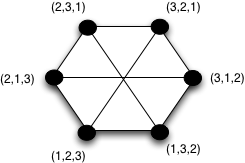
\includegraphics[width=0.6\textwidth]{./images/neighborhood.png}
\caption{ An example of neighborhood for a permutation \cite{Talbi2013}.}
\label{fig:sperneighborhood}
\end{figure}



Single-Solution Based Metaheuristics methods are characterized by a trajectory in the search space. Two common S-metaheuristics methods are Simulated Annealing and Tabu Search.


\subsection{Simulated Annealing}

Simulated Annealing (SA) is a randomized algorithm that tries to avoid being trapped in local optimum solution by assigning probabilities to deteriorating moves. The SA procedure is inspired from the annealing process of solids. SA is based on a physical
process in metallurgy discipline or solid matter physics. Annealing is the process of obtaining low energy states of a solid in heat treatment \cite{Jaziri2008}. 

The algorithmic framework of SA is described in Alg. \ref{sa}.  The algorithm starts by generating an initial solution in function \textit{GenerateInitialSolution()}. The initial temperature value is determined in function \textit{SetInitialTemperature()} such that the probability for an uphill move is quite high at the start of the algorithm. At each iteration a solution $\mbox{s}_1$ is randomly chosen in function \textit{PickNeighborAtRandom(N(s))}. If \textit{$\mbox{s}_1$} is better than \textit{s}, then \textit{$\mbox{s}_1$} is accepted as new current solution. Else, if the move from \textit{s} to \textit{$\mbox{s}_1$} is an uphill move, \textit{$\mbox{s}_1$}  is accepted with a probability which is a function of a temperature parameter \textit{Tk} and \textit{s} \cite{raidl2010metaheuristic}. 

\begin{algorithm}[h]
  \caption{Simulated Annealing Algorithm}\label{sa}
  \begin{algorithmic}[1]
    
    \State $s\gets GenerateInitialSolution()$
    \State $k\gets 0 $
    \State $Tk\gets SetInitialTemperature()$
    \While{termination conditions not met }
    \State $\mbox{s}_1\gets PickNeighborAtRandom(N (s))$
    \If{$(f(\mbox{s}_1)<f(s))$}
    \State $s\gets\mbox{s}_1$
    \Else $\;$ Accept $\mbox{s}_1$ as new solution with probability p($\mbox{s}_1|$Tk,s) 
    \EndIf
    \State $K\gets K+1$
    \State $Tk\gets AdaptTemperature()$
    \EndWhile
      
  \end{algorithmic}
\end{algorithm}

\subsection{Tabu Search}

Tabu Search (TS) is a metaheuristic that guides a local heuristic search procedure to explore the solution space beyond local optimal and search with short term memory to avoid cycles. Tabu Search uses a  tabu list to keep track of the last  moves, and don’t allow going back to these \cite{Glover1986}.

The basic idea of TS is the explicit use of search history, both to escape
from local minima and to implement a strategy for exploring the search space.
A basic TS algorithm uses short term memory in the form of socalled
tabu lists to escape from local minima and to avoid cycles \cite{Tobergte2013}.

The algorithmic framework of Tabu Search is described in Alg. \ref{tsa}.  The algorithm starts by generating an initial solution in function \textit{GenerateInitialSolution()} and the tabu lists are initialized as empty lists in function \textit{InitializeTabuLists($\mbox{TL}_1$,...,$\mbox{TL}_r$)}. For performing a move, the algorithm first determines those solutions from the neighborhood \textit{N(s)} of the current solution \textit{s} that contain solution features currently to be found in the tabu lists. They are excluded from the neighborhood, resulting in a restricted set of neighbors \textit{$\mbox{N}_a(s)$}. At each iteration the best solution \textit{$\mbox{s}_1$} from \textit{$\mbox{N}_a(s)$} is chosen as the new current solution. Furthermore, in procedure \textit{UpdateTabuLists($\mbox{TL}_1$,...,$\mbox{TL}_r$,s,$\mbox{s}_1$)} the corresponding features of this solution are added to the tabu lists.


\begin{algorithm}[h]
  \caption{Tabu Search Algorithm}\label{tsa}
  \begin{algorithmic}[2]
    
    \State $s\gets GenerateInitialSolution()$
    \State InitializeTabuLists($\mbox{TL}_1$,...,$\mbox{TL}_r$)
    \While{termination conditions not met }
    \State $\mbox{N}_a(s)\gets$ $\{\mbox{s}_1 \in N(s) |\mbox{s}_1$ does not violate a tabu condition, or it satisfies at least one aspiration condition $\}$ 
    \State $\mbox{s}_1\gets argmin\{f(\mbox{s}_2)|\mbox{s}_2 \in \mbox{N}_a(s) \}$
    \State UpdateTabuLists($\mbox{TL}_1$,...,$\mbox{TL}_r$,s,$\mbox{s}_1$)
    \State $s\gets \mbox{s}_1$
    \EndWhile
      
  \end{algorithmic}
\end{algorithm}

\section{Population-based metaheuristics}

Population-based metaheuristics (P-metaheuristics) could be viewed as an iterative improvement in a population of solutions. First, the population is initialized. Then, a new population of solutions is generated. Finally, this new population is integrated into the current one using some selection procedures. The search process is stopped when a stopping criterion is satisfied. Algorithms such as Genetic algorithms (GA), scatter search (SS), estimation of distribution algorithms (EDAs), particle swarm optimization (PSO), bee colony (BC), and artificial immune systems (AISs) belong to this class of metaheuristics \cite{talbi2009metaheuristics}. 

\subsection{Genetic Algorithms}

Genetic Algorithms could be a mean of solving complex optimization problems that are often NP Hard. GAs are based on concepts adopted from genetic and evolutionary theories. GAs are comprised of several components \cite{hong2000simultaneously} \cite{shousha2003performance} :

\begin{itemize}
\item a representation of the solution, refered as the chromossome;
\item fitness of each chromossome, refered as objective function;
\item the genetic operations of crossover and mutation which generate new offspring. 
\end{itemize}


Algorithm \ref{gna} shows the basic structure of GA algorithms. In this algorithm, P denotes the population of individuals. A population of offspring is generated by the application of recombination and mutation operators and the individuals for the next population are selected from the union of the old population and the offspring population \cite{raidl2010metaheuristic}.


\begin{algorithm}[h]
  \caption{Genetic Algorithm}\label{gna}
  \begin{algorithmic}[3]
    
    \State $s\gets GenerateInitialSolution()$
    \State Evaluate(P)
    \While{termination conditions not met }
    \State $\mbox{P}_1\gets$ $Recombine(P)$
    \State $\mbox{P}_2\gets$ $Mutate(\mbox{P}_1)$ 
    \State $Evaluate(\mbox{P}_2)$
    \State $P\gets Select(\mbox{P}_2,P)$
    \EndWhile
      
  \end{algorithmic}
\end{algorithm}

\section{Hybrid  Metaheuristics}

However, in recent years it has become evident that the concentration on a sole metaheuristic is rather restrictive. A skilled combination of a metaheuristic with other optimization techniques, a so called hybrid metaheuristic, can provide a more efficient behavior
and a higher flexibility when dealing with real-world and large-scale problems \cite{Talbi2012}.

A combination of one metaheuristic with components from other metaheuristics is called a hybrid metaheuristic. The concept of hybrid metaheuristics has been commonly accepted only in recent years, even if the idea of combining different metaheuristic strategies and algorithms dates back to the 1980s. Today, we can observe a generalized common agreement on the advantage of combining components from different search techniques and the tendency of designing hybrid techniques is widespread in the fields of operations research and artificial intelligence \cite{raidl2010metaheuristic}. 


There are two main categories of metaheuristic combinations: collaborative combinations and integrative combinations. These are presented in Fig. \ref{fig:metaheuristc} \cite{Raidl2006}.

\begin{figure}[h]
\centering
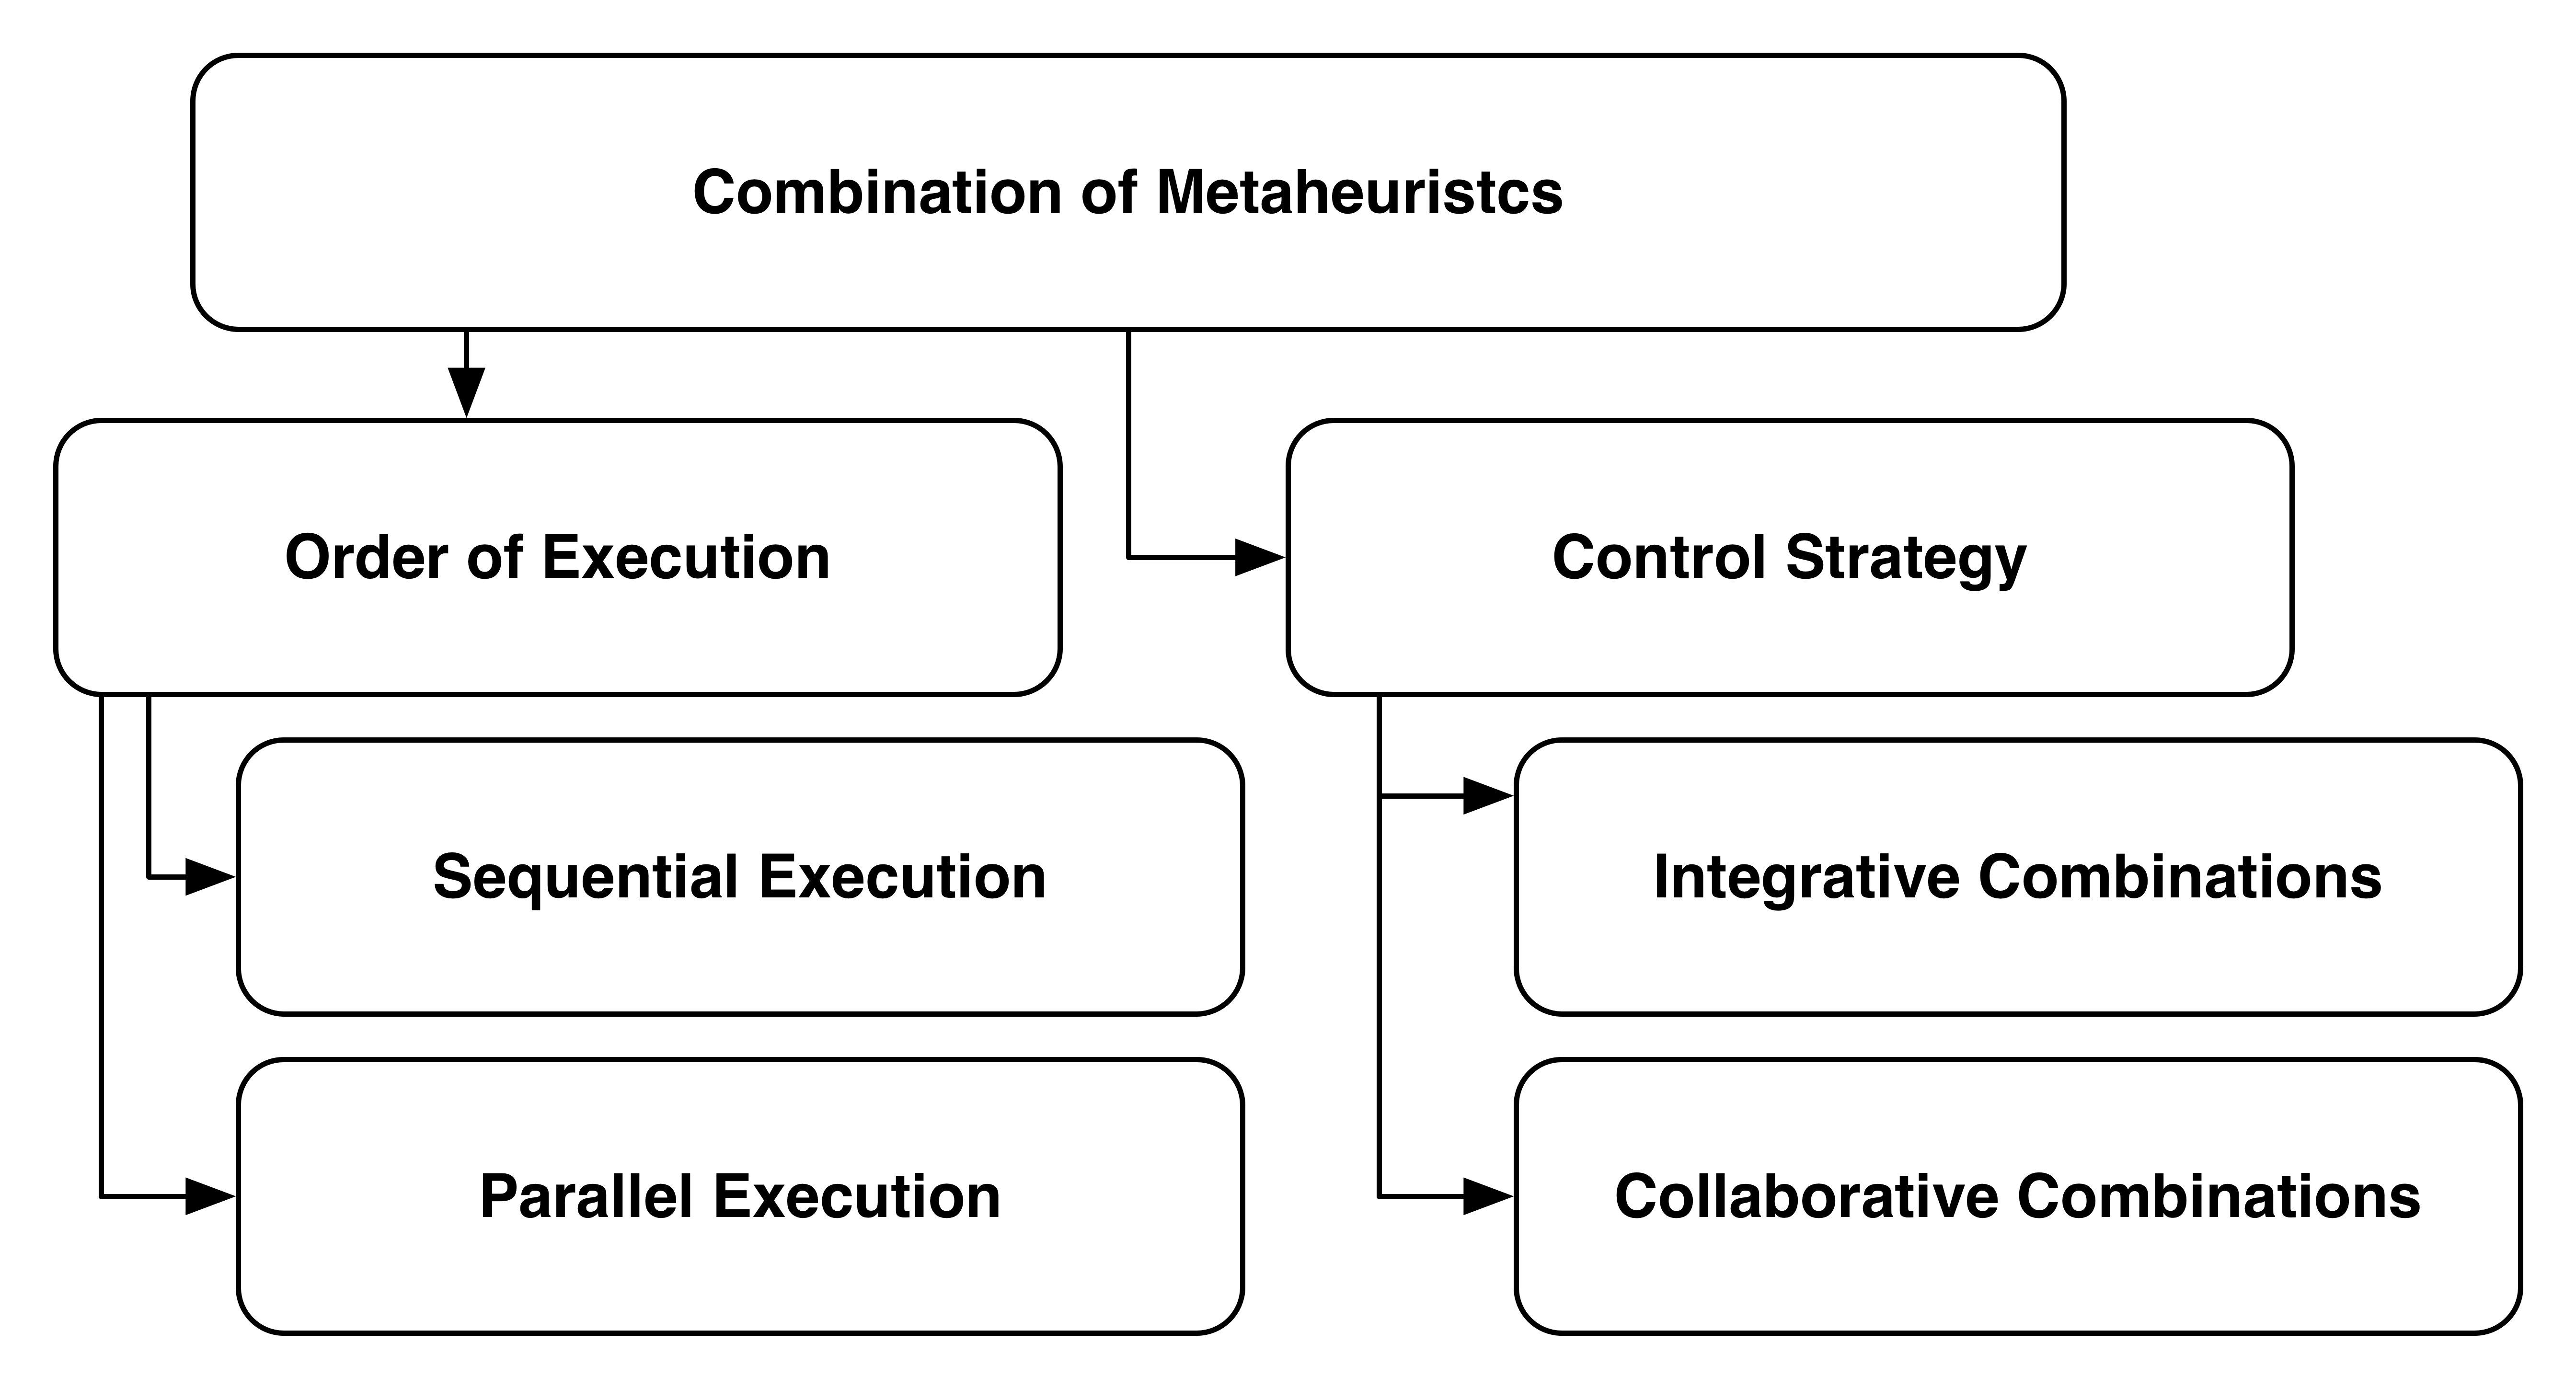
\includegraphics[width=1\textwidth]{./images/metaheuristc2.png}
\caption{Categories of metaheuristc combinations \cite{Puchinger2005} }
\label{fig:metaheuristc}
\end{figure}

Collaborative combinations use an approach where the algorithms exchange information, but are not part of each other. In this approach, algorithms may be executed sequentially or in parallel. 

One of the most popular ways of metaheuristic hybridization consists in the use of trajectory methods inside population-based methods. Population-based methods are better in identifying promising areas in the search space from which trajectory methods can quickly reach good local optima. Therefore, metaheuristic hybrids that can effectively combine the strengths of both population-based methods and trajectory methods are often very successful \cite{raidl2010metaheuristic}.


The work uses a type of collaborative combination with sequential execution with two trajectory methods (Tabu Search and Simulated Annealing) and Genetic Algorithms.





\section{Q-Learning}




\subsection{Reinforcement Learning}

Reinforcement learning (RL) refers to both a learning problem and a subfield of machine
learning. As a learning problem, it refers to learning to control a system so as to maximize
some numerical value which represents a long-term objective. A typical setting where
reinforcement learning operates is shown in Figure \ref{fig:agentenv}: A controller receives the controlled
system’s state and a reward associated with the last state transition. It then calculates an
action which is sent back to the system.


\begin{figure}
\centering
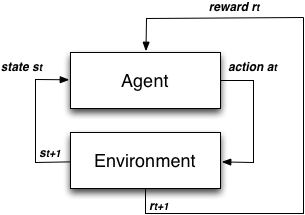
\includegraphics[width=0.7\textwidth]{./images/agentenv.png}
\caption{Example of interation between some agent and the environment}
\label{fig:agentenv}
\end{figure}


The basis idea of Reinforcement learning  is simply to capture the most important aspects of the real problem facing a learning agent interacting with its environment to achieve a goal \cite{Sutton2012}. Reinforcement learning is learning what to do—how to map situations to actions—so as to maximize a numerical reward signal. The learner need to discover which actions yield the most reward by trying them \cite{Sutton2012}.

In Reinforcement Learning, an agent wanders in an unknown environment and tries to maximize its long term return by performing actions and receiving rewards. The challenge is to understand how a current action will affect future rewards. A good way to model this task is with Markov Decision Processes (MDP), which have become the dominant approach in Reinforcement Learning. There are two types of learning problems:

\begin{itemize}
\item Iteractive learning;
\item Non-interactive learning.
\end{itemize}

In non-interactive learning, the natural goal is to find a good policy given a fixed number of observations. A common situation is when the sample is fixed. For example, the sample can be the result of some experimentation with some physical system that happened before learning started. 

In Interactive learning, learning happens while interacting with a real system in a closed-loop fashion. A reasonable goal then is to optimize online performance,
making the learning problem an instance of online learning. Online performance can be measured in different ways. A natural measure is to use the sum of rewards incurred during learning. 

Interactive learning is potentially easier since the learner has the additional option to influence the distribution of the sample. However, the goal of
learning is usually different in the two cases, making these problems incomparable in general.

In Reinforcement Learging, all agents act in two phases: Exploration vs Explotation. In Exploration phase, the agents tries discover better action selections to improve its knowledge. In Explotation phase, the agents tries to maximize its reward, based on what its already know.

One of the challenges that arise in reinforcement learning is the trade-off between exploration and exploitation. To obtain a lot of reward, a reinforcement learning
agent must prefer actions that it has tried in the past and found to be effective in producing reward.
But to discover such actions, it has to try actions that it has not selected before. The agent has to exploit what it already knows in order to obtain reward, but it also has to explore in order to make better action selections in the future.





\subsection{Markov decision processes}

Markov decision processes (MDPs) provide a mathematical framework for modeling decision making. A countable MDP is defined as a triplet $M=(\chi,A,P_{0})$ \cite{Szepesvari2010}. where $\chi$ is a set of states, A is a set of actions. The transition probability kernel $P_{0}$ assigns to each state-action pair $(x, a) \in \chi x A $


The six main elements of a MDP are:(1) state of the system, (2) actions, (3) transition probabilities, (4) transition rewards, (5) a policy, and (6) a performance metric \cite{Sutton2012}.

\begin{figure}
\begin{minipage}{.5\textwidth}
\centering
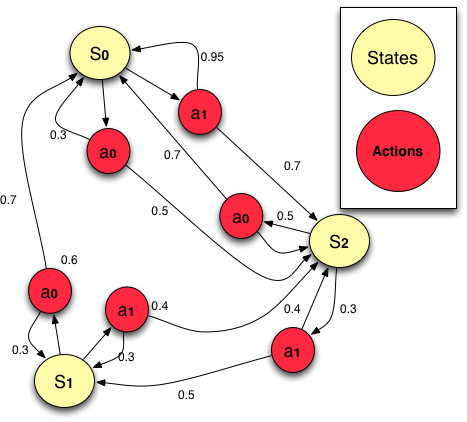
\includegraphics[width=1\textwidth]{./images/mdp1.png}
\caption{Example of a simple MDP with three states and two actions}
\label{fig:mdp}
\end{minipage}
\begin{minipage}{.5\textwidth}
\centering
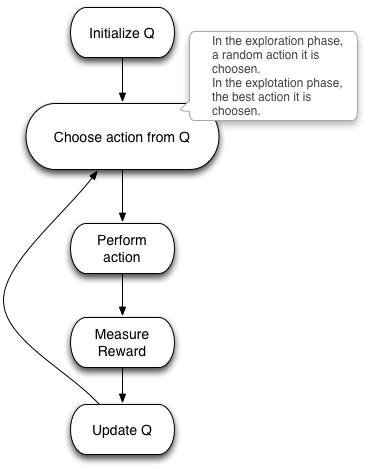
\includegraphics[width=0.8\textwidth]{./images/qalgo.png}
\caption{Q Learning algorithm}
\label{fig:qalgo}
\end{minipage}
\end{figure}



The state of a system is a parameter or a set of parameters that can be used to describe a system. For example the geographical coordinates of a robot can be used to
describe its state. A system whose state changes with time is called a dynamic system. Then it is not hard to see why a moving robot produces a dynamic system.

Actions are the controls allowed for an agent. Transition Probability denotes the probability of going from state i to state j under the influence of action a in one step. If an MDP has 3 states and 2 actions, there are 9 transition probabilities per action. Usually, the system receives an immediate reward ,which could be positive or negative, when it transitions from one state to another

A policy defines the learning agent’s way of behaving at a given time. Roughly speaking, a policy is a mapping from perceived states of the environment
to actions to be taken when in those states. It corresponds to what in
psychology would be called a set of stimulus–response rules or associations.  Policys mapping from states to actions.

Performance Metric: Associated with any given policy, there exists a so-called performance
metric — with which the performance of the policy is judged. Our goal is to select the policy
that has the best performance metric. 


\subsection{Q-Learning}

Q-learning is a model-free reinforcement learning technique. Q-learning, it is a multiagent learning algorithm that learns equilibrium policies in Markov games, just as Q-learning learns to optimal policies in Markov decision processes \cite{Greenwald2003}. 

Q-learning and related algorithms tries to learn the optimal policy from its history of interaction with the environment. A history of an agent is a sequence of state-action-rewards.Where $s_{n}$ it is a state, $a_{n}$ it is an action and $r_{n}$ is a reward:

\begin{equation}
<s_{0},a_{0},r_{1},s_{1},a_{1},r_{2},s_{2},a_{2},r_{3},s_{3},a_{3},r_{4},s_{4}....>,
\end{equation}


In Q-Learning, the system's objective is to learn a control policy $\pi = \sum_{n=0}^{\infty} \gamma\textsuperscript{n}  r_{t}+n $, where $\pi$  is the discounted cumulative reward, $\gamma$ is the discount rate ($01$) and $r_{t}$ is the reward reiceved after execution an action at time t. The fig. \ref{fig:qalgo} shows the summary version of Q-Learning algorithm. The first step it is to generate the initial state of the MDP. The second step it is to choose the best action or a random action based on the reward, the actions with best rewards are chosen.




\subsection{GridWorld Example}

The GridWorld problem is an example of using reinforcement learning with Q-Learning. In this example,  The agent's goal is to reach the reward state.  There are one rewarding states with value +1 (Gray square at position (3,1)). The agent receives +0.02 of reward if it get closer to the reward state  As the agent moves away from the reward state, he receives -0.01 of reward.The agente receive +0 points of reward if it is the same distance to the reward state.

The Fig. \ref{fig:gridworld} shows the initial and final phase on exploration phase. The numbers in the squares shows the Q-values  for four available actions: up (u), left (l), right(r) and down(d). The arrows show the optimal action based on the current value function. The initial discount rate is 0.9. 

\begin{figure}[h!]
\centering
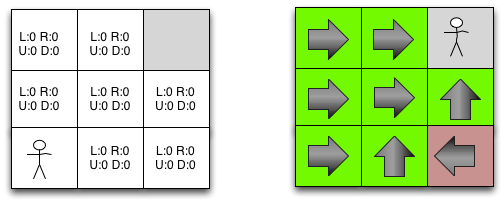
\includegraphics[width=1\textwidth]{./images/mdpgridworld.png}
\caption{GridWorld - initial and final stage on exploration phase}
\label{fig:gridworld}
\end{figure}

The figure  \ref{fig:gridworld1},\ref{fig:gridworld2}, \ref{fig:gridworld3} and \ref{fig:gridworld4}   shows the states of the game in exploration phase. In the first image, all frames have the accumulated reward value equals to zero. In the next images the reward values increase or decrease as the agent moves.

\section{Relationships Between Reinforcement Learning and Optimization}

Many are the intersections between optimization and Reinforcement Learning. First, approximated versions of optimazation and RL tasks contain challenging optimization tasks,  the maximization operations in determining the best action when an action value function is available or the optimal choice of approximation \cite{Battiti2009}. Both optimization and Machine Learning analysts address real world problems by formulating a model, deriving the core optimization problem, and using mathematical programming to solve it \cite{Bennett2006} \cite{Boyan2000}. 

Gambardella et al. show an Ant metaheuristic with Q-Learning approach (Ant-Q). They experimentally investigate the functioning of Ant-Q and we show that the results obtained by Ant-Q on symmetric TSP's are competitive with those obtained by other heuristic approaches based on neural networks or
local search. The research used Q-Learning to indicate how useful it is to make move in TSP for each ant \cite{Gambardella1995}.  Bianchi et at.  present a new algorithm, called Heuristically Accelerated Q–Learning (HAQL), that allows the use of heuristics to speed up the well-known Reinforcement Learning algorithm Q–learnin    g. The Heuristically Accelerated Q–Learning algorithm can be defined as a way of solving the RL problem which makes explicit use of a heuristic function to influence the choice of actions during the learning process. The HAQL uses a modification Greedy rule to control exploration and exploitation phases \cite{Matsuura2015}. 

\section{Software Testing with Reinforcement Learning}

Many software systems are reactive. The behavior of a reactive system, especially when distributed or multithreaded, can be nondeterministic. In these cases, a test suite generated offline may be infeasible.

Online testing is a formal model-based testing (MBT),where the tester uses a specification of the system's behavior to guide the testing and to detect the discrepancies between the aplication under test and the model.Online testing can be more appropriate than offline tests for reactive systems. The reason is that with online testing the tests may be dynamically adapted at runtime, effectively pruning the search space to include only those behaviors actually observed instead of all possible behaviors. The interaction between tester and the application under test is seen as a game  where the tester chooses moves based on the observed behavior of the implementation under test \cite{Havelund2006}.

Havelund et al transforms online testing problem into a special case of reinforcement learning where the frequencies of various abstract behaviors are recorded and allows to better choose controllable actions \cite{Havelund2006}.

Andre et al. show a method that operationalizes the risk assessment for interoperability testing. Typically high number of possible interaction scenarios makes interoperability testing a complex task. Since it seems impossible to cover all scenarios, their relevance for being tested has to be prioritized. The method uses behavior models of the system under test and reinforcement learning techniques to obtain the relevance of single system actions for being tested \cite{Piel2010}. The table \ref{tab:testq1} shows the Q-value for some states of the test. 


% Please add the following required packages to your document preamble:
% \usepackage[table,xcdraw]{xcolor}
% If you use beamer only pass "xcolor=table" option, i.e. \documentclass[xcolor=table]{beamer}
\begin{table}[h]
\centering
\caption{Q-value for some states of the test \cite{Piel2010}}
\label{tab:testq1}
\begin{tabular}{lll}
\rowcolor[HTML]{C0C0C0} 
\textbf{State} & \textbf{Action} & \textbf{Q-value} \\
M'1N1O1       & M 1 → M 2       & 2.5              \\
M'2N2O2       & M 2 → M 1       & 1.25             \\
M'2N2O2       & M 2 → M 3       & 0.0              \\
M'1N1O2       & M 1 → M 2       & 0.5             
\end{tabular}
\end{table}


Sato and Sugihara propose an automatic test pattern generation by applying genetic algorithms in reinforcement learning. The results of evaluation with an ATM system which assuming the existence of a bug related to a global variable are reported \cite{sato2015automatic}. 

Meinke and Niu presents an application of learning techniques to the problem of automated test case generation for numerical software. Our approach uses n-dimensional polynomial models as an algorithmically learned abstraction of the application under test. Test cases are iteratively generated by applying a satisfiability algorithm to first-order program specifications over real closed fields and iteratively refined piecewise polynomial models \cite{Meinke2010}. Kamali et al. propose a  approach based on Q-learning, on top of genetic algorithms (GA) to determine the best weightings for an metaheuristic \cite{Kamali2007}.


\section{Improving Stress Search Based Testing using Q-Learning and Hybrid Metaheuristic Approach}


\subsection{Hybrid Approach}

A large number of researchers have recognized the advantages and huge potential of building hybrid metaheuristics. The main motivation for creating hybrid metaheuristics is to exploit the complementary character of different optimization strategies. In fact, choosing an adequate combination of algorithms can be the key to achieving top performance in solving many hard optimization problems \cite{Puchinger2005} \cite{Blum2012}.

The proposed solution makes it possible to create a model that evolves during the test. The proposed solution model uses genetic algorithms, tabu search, and simulated annealing in two different approaches. The study initially investigated the use of these three algorithms. Subsequently, the study will focus in others Population-based and single point search metaheuristics. The first approach uses the three algorithms independently, and the second approach uses the three algorithms collaboratively (hybrid metaheuristic approach).

In the first approach , the algorithms do not share their best individuals among themselves. Each algorithm evolves in a separate way (Fig. \ref{fig:firstaproach}).





The second approach uses the algorithms in a collaborative mode (hybrid metaheuristic). In this approach, the three algorithms share their best individuals found (Fig. \ref{fig:secondapproach}). The next subsections present details about the used metaheuristic algorithms (Representation, initial population and fitness function). The exp



\begin{figure}[h]
\begin{minipage}{.5\textwidth}
\centering
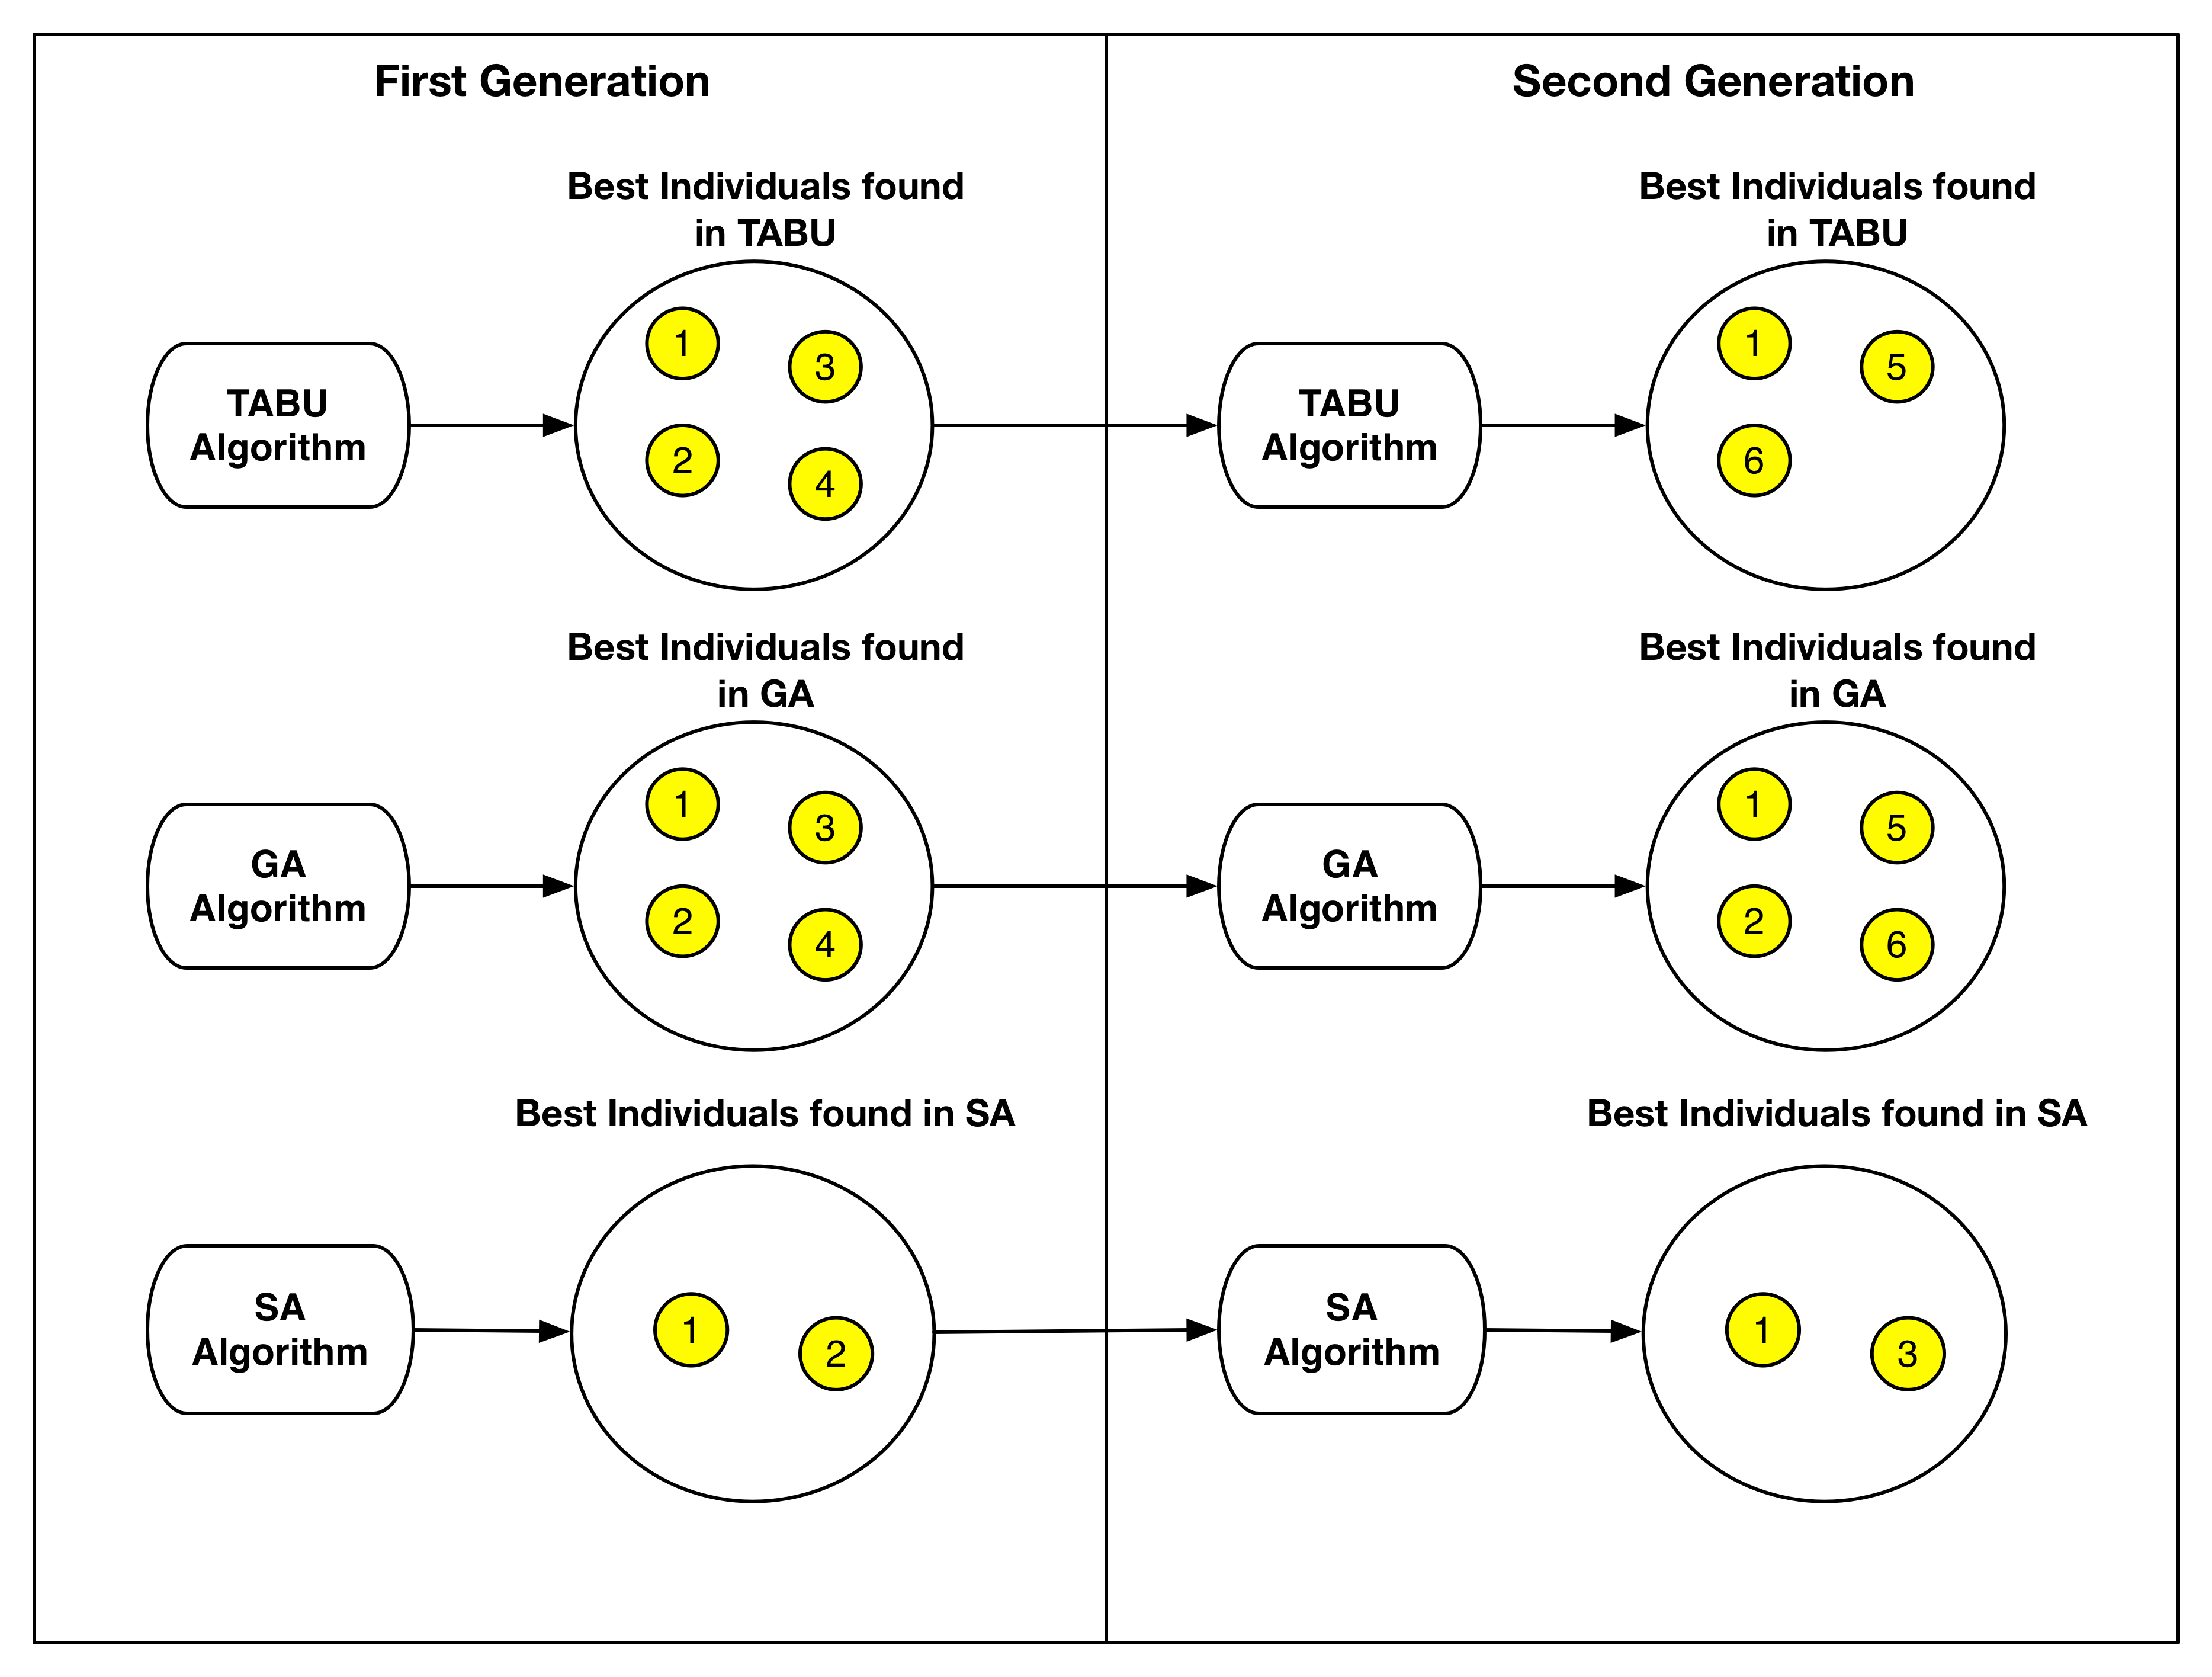
\includegraphics[width=1\textwidth]{./images/independ.png}
\caption{Use of the algorithms independently}
\label{fig:firstaproach}
\end{minipage}
\begin{minipage}{.5\textwidth}
\centering
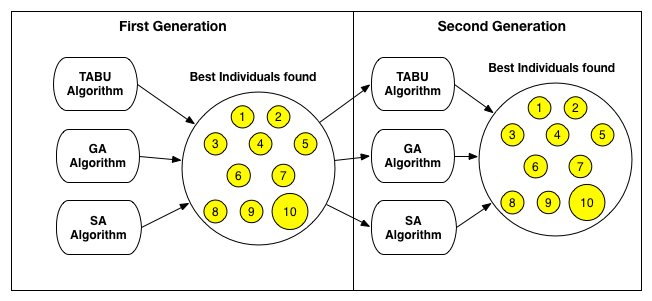
\includegraphics[width=1\textwidth]{./images/collaborative.png}
\caption{Use of the  algorithms collaboratively}
\label{fig:secondapproach}
\end{minipage}
\end{figure}

\subsubsection{Representation}

The solution representation is composed by a linear vector with 23 positions. The first position represents the name of an individual. The second position represents the algorithm (genetic algorithm, simulated annealing, or Tabu search) used by the individual. The third position represents the type of test (load, stress, or performance). The next positions represent 10 scenarios and their numbers of users. Each scenario is an atomic operation: the scenario must log into the application, run the task goal, and undo any changes performed, returning the application to its original state.

Fig. \ref{fig:genomarepresentation} presents the solution representation and an example using the crossover operation. In the example, genotype 1 has the Login scenario with 2 users, the Form scenario with 0 users, and the Search scenario with 3 users. Genotype 2 has the Delete scenario with 10 users, the Search scenario with 0 users, and the Include scenario with 5 users. After the crossover operation, we obtain a genotype with the Login scenario with 2 users, the Search scenario with 0 users, and the Include scenario with 5 users.

\begin{figure}[h]
\begin{minipage}{.5\textwidth}
\centering
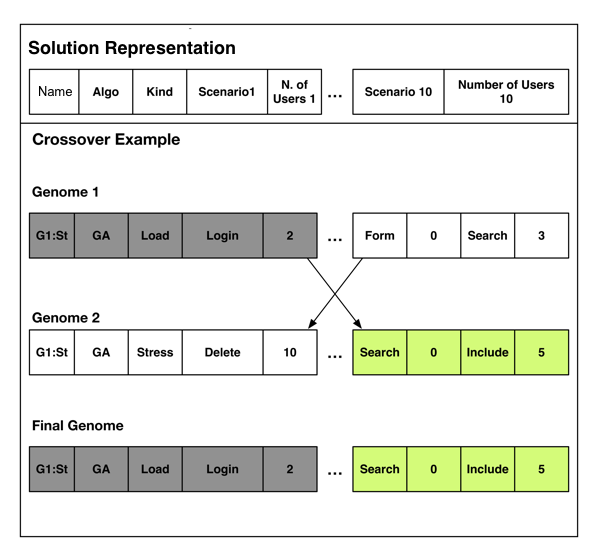
\includegraphics[width=1\textwidth]{./images/genomerepresentation1.png}
\caption{Solution representation and crossover example}
\label{fig:genomarepresentation}
\end{minipage}
\begin{minipage}{.5\textwidth}
\centering
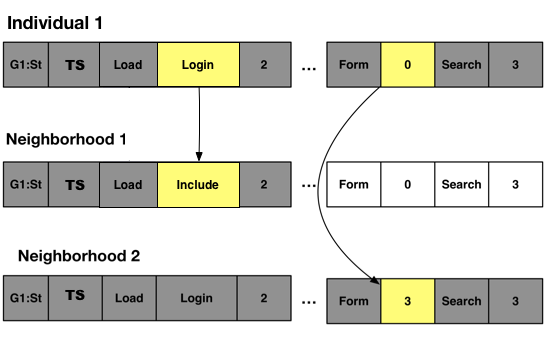
\includegraphics[width=1\textwidth]{./images/neighbor.png}
\caption{Tabu search and simulated annealing neighbor strategy}
\label{fig:neighbourtaby}
\end{minipage}
\end{figure}

Fig. \ref{fig:neighbourtaby} shows the strategy used by the proposed solution to obtain the representation of the neighbors for the Tabu search and simulated annealing algorithms. The neighbors are obtained by the modification of a single position (scenario or number of users) in the vector.





\subsubsection{Initial population}

The strategy used by the plugin to instantiate the initial population is to generate 50\% of the individuals randomly, and 50\% of the initial population is distributed in three ranges of values:

\begin{itemize}
\item Thirty percent of the maximum allowed users in the test;
\item Sixty percent of the maximum allowed users in the test; and
\item Ninety percent of the maximum allowed users in the test.
\end{itemize}

The percentages relates to the distribution of the users in the initial test scenarios of the solution. For example, in a hypothetical test with 100 users, the solution will create initial test scenarios with 30, 60 and 90 users.

\subsubsection{Objective (fitness) function}

The proposed solution was designed to be used with independent testing teams in various situations where the teams have no direct access to the environment where the application under test was installed. Therefore, the IAdapter plugin uses a measurement approach to the definition of the fitness function. The fitness function applied to the IAdapter solution is governed by the following equation:

\begin{equation}
\begin{aligned}
fit=90percentileweigth* 90percentiletime\\
+80percentileweigth*80percentiletime\\+
70percentileweigth*70percentiletime+\\
maxResponseWeigth*maxResponseTime+\\
numberOfUsersWeigth*numberOfUsers-penalty
\end{aligned}
\end{equation}

The proposed solution's fitness function uses a series of manually adjustable user-defined weights (90percentileweight, 80percentileweight,  70percentileweight, maxResponseWeight, and numberOfUsersWeight). These weights make it possible to customize the search plugin's functionality. A penalty is applied when an application under test takes a longer time to respond than the level of service. The penalty is calculated by the follow equation:

\begin{equation}
\begin{aligned}
penalty=100 * \Delta \\
\Delta=(t_{Current Response Time} - t_{Maximum Response Time Expected})\\
\end{aligned}
\end{equation}

\subsection{Hybrid Metaheuristic with Q-Learning Approach}

The HybridQ algorithm uses the GA, SA and Tabu Search algorithms in a collaborative approach in conjunction with Q-Learning technique. The biggest difference between the Hybrid and HybridQ algorithms is the application of a series of modifications on individuals based on the Q-Learning algorithm before each generation.

\begin{figure}[h!]
\center
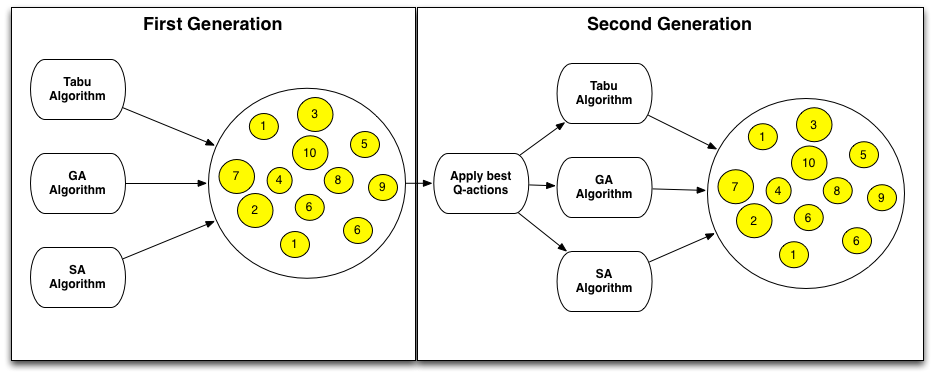
\includegraphics[width=1\textwidth]{./images/qhybrid.png}
\caption{Hybrid Metaheuristic with Q-Learning Approach}
\label{fig:hybridq}
\end{figure}

Figure \ref{fig:mdphybridq} shows the proposed MDP model for HybridQ. The model has three main states based on response time. A test may have a response time greater than 1.2 times the maximum response time alloowed, between 0.8 and 1.2 times the maximum response time allowed or less than 0.8 times the maximum response time allowed. A test receives a positive reward when an action increases fitnesse value and a negative reward when an action reduces the fitnesse value. The possible actions in MDP are the change of one of the test scenarios and increase or decrease of the number of users.

\begin{figure}[h!]
\begin{minipage}{.5\textwidth}
\center
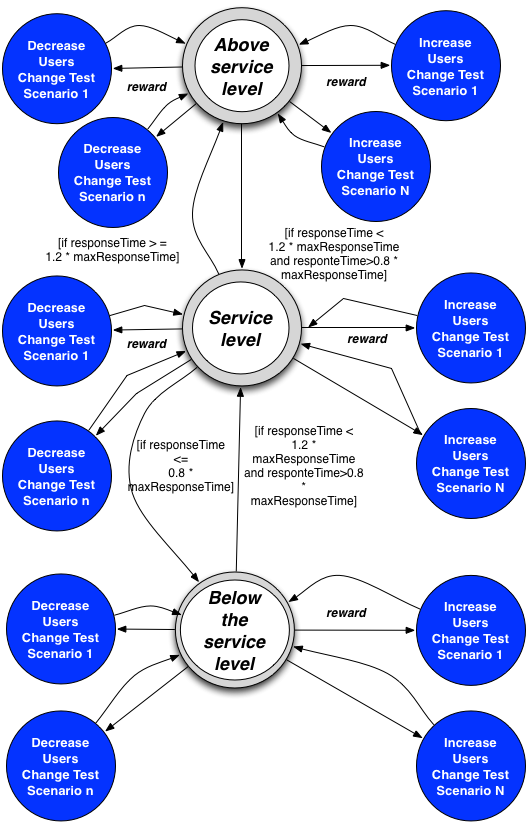
\includegraphics[width=1\textwidth]{./images/mdp3.png}
\caption{Markov Decision Process used by HybridQ}
\label{fig:mdphybridq}
\end{minipage}
\begin{minipage}{.5\textwidth}
\center
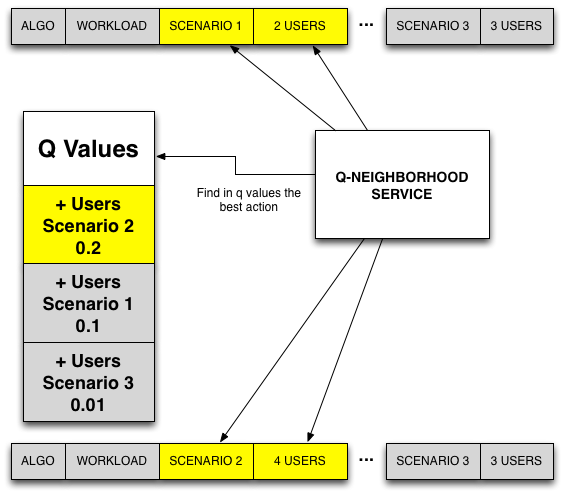
\includegraphics[width=1\textwidth]{./images/q-neighborservice.png}
\caption{HybridQ NeighborHood Service}
\label{fig:neighservice}
\end{minipage}
\end{figure}



Unlike the traditional approach, The update of Q values for each action also occurs in the explotation phase. The exploit phase ends when no value of Q it is equals zero for a state, ie, unlike the traditional approach an agent belonging to one state may be in the exploration phase while another agent may be in the explotation phase. The table presents an hyphotetical Q-values for a test. In the table \ref{pab:mdp}, it can be observed that the agents in the Service Level state are in the exploitation phase because there is no other value of Q equals to zero.


% Please add the following required packages to your document preamble:
% \usepackage[table,xcdraw]{xcolor}
% If you use beamer only pass "xcolor=table" option, i.e. \documentclass[xcolor=table]{beamer}
\begin{table}[]
\centering
\caption{Hypothetical MDP Q-values }
\label{pab:mdp}
\begin{tabular}{lll}
\rowcolor[HTML]{C0C0C0} 
\textbf{Above Service Level}  & \textbf{Scenario 1} & \textbf{Scenario 2} \\
Increment Users               & 0.2                 & 0.0                 \\
Reduce Users                  & 0.1                 & 0.2                 \\
Phase                         & Exploration         & Exploration         \\
\rowcolor[HTML]{C0C0C0} 
\textbf{Service Level}        & \textbf{Scenario 1} & \textbf{Scenario 2} \\
Increment Users               & 0.2                 & 0.11                \\
Reduce Users                  & 0.1                 & -0.2                \\
\rowcolor[HTML]{F8FF00} 
Phase                         & Explotation         & Explotation         \\
\rowcolor[HTML]{C0C0C0} 
\textbf{Bellow Service Level} & \textbf{Scenario 1} & \textbf{Scenario 2} \\
Increment Users               & 0.0                 & 0.2                 \\
Reduce Users                  & 0.1                 & 0.0                 \\
Phase                         & Exploration         & Exploration        
\end{tabular}
\end{table}

The Fig. \ref{fig:neighservice} presents how one of the neighbors of a test is generated using Q-Learning. The solution uses a service called Q-Neighborhood Service to generate the neighbor from the action that has the highest value of Q.




\subsection{IAdapter}

IAdapter is a JMeter plugin designed to perform search-based stress tests.  The plugin is available on www.iadapter.org.  The IAdapter plugin implements the solution proposed in Section 5. The next subsections present details about the Apache JMeter tool, the IAdapter Life Cycle and the IAdapter Components. The IAdapter plugin provides three main components: WorkLoadThreadGroup, WorkLoadSaver, and WorkLoadController.

The Fig. \ref{fig:iadapterarchitecture} show the IAdapter architecture. All metaheuristic class implements the interface IAlgorithm. Test scenarios  and test results are stored in a Mysql database. GeneticAlgorithm class uses a framework named JGAP to implement Genetic Algorithms.

\begin{figure}[h]
\begin{minipage}{.5\textwidth}
\center
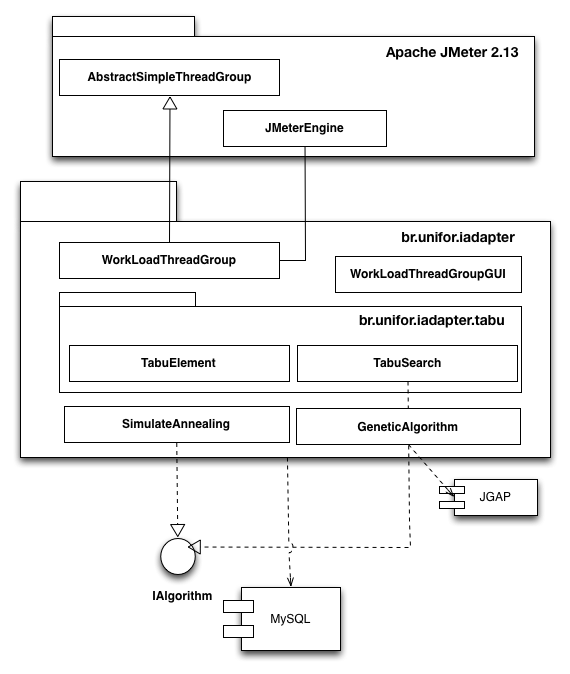
\includegraphics[width=1\textwidth]{./images/iadapter1.png}
\caption{IAdapter architecture}
\label{fig:iadapterarchitecture}
\end{minipage}
\begin{minipage}{.5\textwidth}
\centering
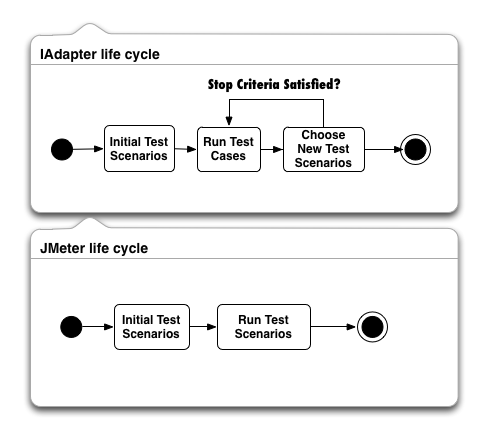
\includegraphics[width=1\textwidth]{./images/lifecycle2.png}
\caption{IAdapter life cycle}
\label{fig:iadapterlifecycle}
\end{minipage}
\end{figure}

The WorkLoadThreadGroup class is the Load Injection and Test Management modules, responsible to generate the initial population and uses the JMeter Engine to realize requests to server under test. 

\subsubsection{IAdapter Life Cycle}
 
Fig. \ref{fig:iadapterlifecycle} presents the IAdapter Life Cycle. The main difference between IAdapter and JMeter tool is that the IAdapter provide an automated test execution where the new test scenarios are choosen by the test tool.  In a test with JMeter, the tests scenarios are usually chosen by a test designer.



\subsubsection{IAdapter Components}
 
WorkLoadThreadGroup is a component that creates an initial population and configures the algorithms used in IAdapter. Fig. \ref{fig:tela1iadapter} presents the main screen of the WorkLoadThreadGroup component. The component has a name \ding{202}, a set of configuration tabs \ding{203}, a list of individuals by generation \ding{204}, a button to generate an initial population \ding{205}, and a button to export the results \ding{206}.

\begin{figure}[h]
\centering
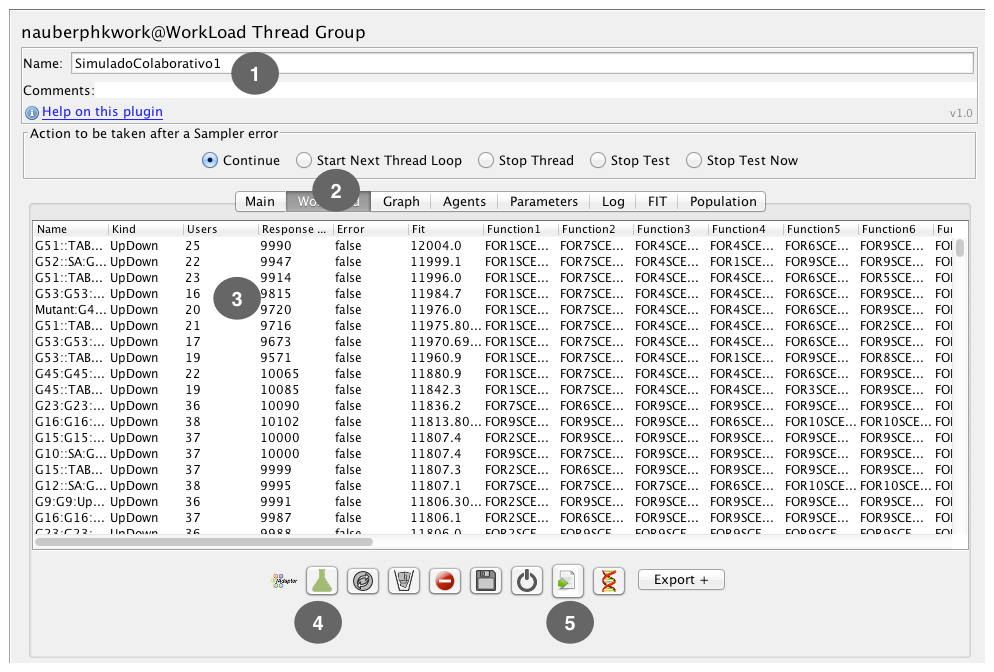
\includegraphics[width=0.8\textwidth]{./images/tela1iadapter.png}
\caption{WorkLoadThreadGroup component}
\label{fig:tela1iadapter}
\end{figure}

WorkLoadThreadGroup component uses the GeneticAlgorithm, TabuSearch and SimulateAnnealing classes.  The WorkLoadSaver component is responsible for saving all data in the database. The operation of the component only requires its inclusion in the test script.

WorkLoadController represents a scenario of the test. All actions necessary to test an application should be included in this component. All instances of the component need to login into the application under test and bring the application back to its original state.

\section{Experiments}

We conducted three experiments in order to verify the effectiveness of the HybridQ. The first two experiments ran for 17 generations in an emulated evinronment. The experiments used an initial population of 4 individuals by metaheuristic. The genetic algorithm used the top 10 individuals from each generation in the crossover operation. The Tabu list was configured with the size of 10 individuals and expired every 2 generations.  The mutation operation was applied to 10\% of the population on each generation. The experiments uses tabu search, genetic algorithms and the hybrid metaheuristic approach proposed by Gois et al. \cite{Gois2016} and the HybridQ approach. 


The objective function applied is intended to maximize the number of users and minimize the response time of the scenarios being tested.  In this experiments, better fitness values meaning to find scenarios with more users and a low values of response time. A penalty is applied when the response time is greater than the  maximum response time expected. The experiments used the following fitness (goal) function. :

\begin{equation}
\begin{aligned}
fitness=3000*numberOfUsers\\
-20* 90percentiletime\\
-20*80percentiletime\\
-20*70percentiletime\\
-20*maxResponseTime\\
-penalty
\end{aligned}
\end{equation}

The experiments addresses:

\begin{itemize}
\item Validate the operation of the testbed tool.
\item Find the maximum number of users and the minimal response time.
\item Analyze and verify the best heuristics among those chosen to the experiments.
\end{itemize}


\subsection{Hybrid-Q Second Experiment}

The experiment was carried out for 8 continuous hours.  All tests in the experiment were conducted without the need of a tester, automating the process of executing and designing performance test scenarios.In this experiment, Scenarios were generated with the Ramp and Circuitous Treasure antipattern as well as scenarios with Happy Scenario 1, Happy Scenario 2 and mixed scenarios. The Fig. \ref{fig:fitnessbygeneration1}  presents the fitness value obtained by each metaheuristic. HybridQ metaheuristic obtained the better fitness values. 


\begin{figure}[H]
\begin{minipage}{.5\textwidth}
\centering
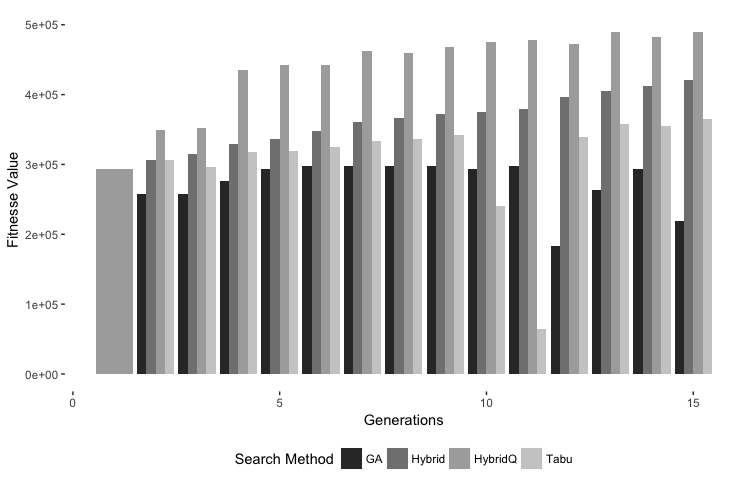
\includegraphics[width=0.7\textwidth]{./images/experiment1-1.png}
\caption{fitness value obtained by Search Method }
\label{fig:fitnessbygeneration1}
\end{minipage}
\begin{minipage}{.5\textwidth}
\centering
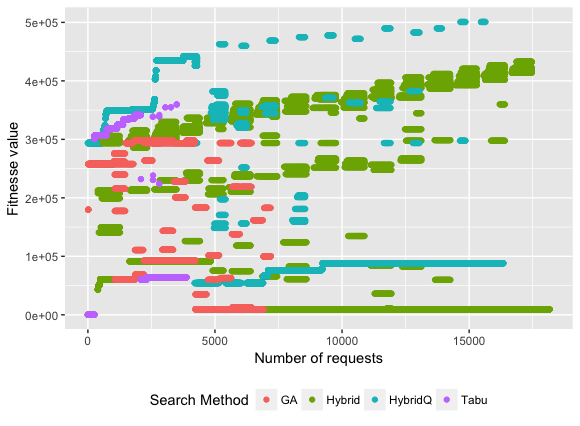
\includegraphics[width=0.8\textwidth]{./images/experiment1-3.png}
\caption{Number of requests by Search Method}
\label{fig:numberofrequestsbysearchmethod}
\end{minipage}
\end{figure}




Despite having obtained the best fitness value in each generation, the Hybrid algorithm performs twice as many requests as the  tabu search (Fig. \ref{fig:numberofrequestsbysearchmethod}). The HybridQ algorithm obtained the best fitness value The Fig. \ref{fig:boxplot1} shows the average, minimal e maximum value by search method.



\begin{figure}[H]
\centering
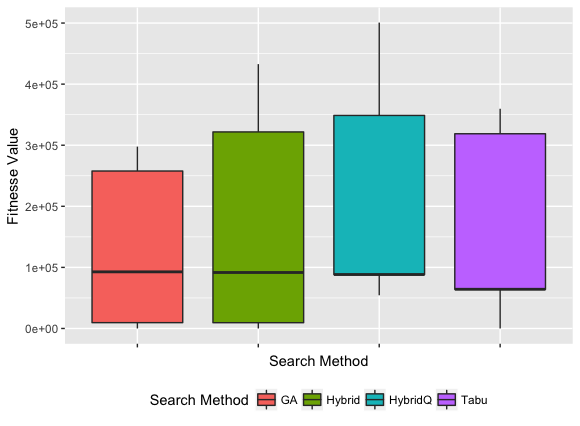
\includegraphics[width=0.8\textwidth]{./images/experiment1-4.png}
\caption{Average, median, maximum and minimal fitness value by Search Method}
\label{fig:boxplot1}

\end{figure}

The Fig. \ref{fig:summaryboxplot1} presents the maximum, average, median and minimum fitness value by generation. The maximun fitness value increases at each generation. The Fig. \ref{fig:density1} presents the density graph of number of users by fitness value. The range between 100 and 150 users has the highest number of individuals found with higher fitness value.

\begin{figure}[H]
\begin{minipage}{.5\textwidth}
\centering
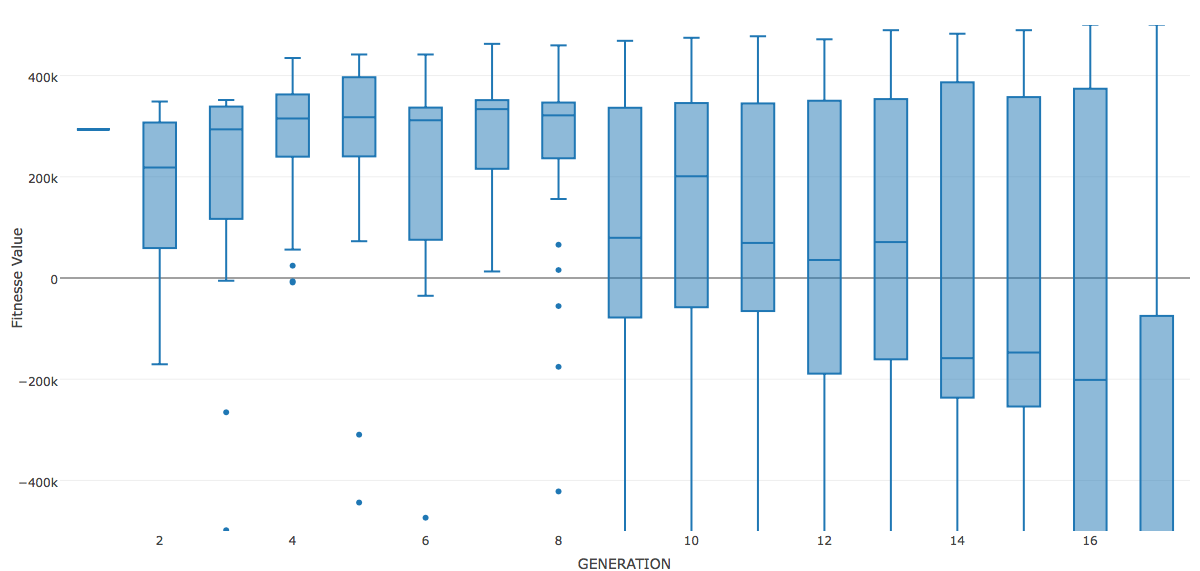
\includegraphics[width=1\textwidth]{./images/experiment1-5.png}
\caption{fitness value by generation}
\label{fig:summaryboxplot1}
\end{minipage}
\begin{minipage}{.5\textwidth}
\centering
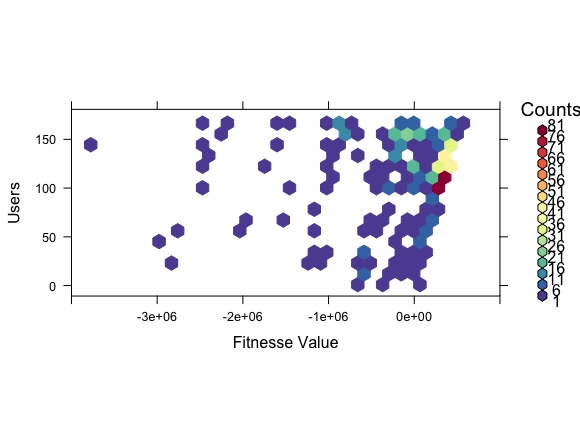
\includegraphics[width=1\textwidth]{./images/experiment1-6.png}
\caption{Density graph of number of users by fitness value}
\label{fig:density1}
\end{minipage}
\end{figure}

Table \ref{tab:bestindividuals} shows 4 individuals with 164 to 169 users. These are the scenarios with the maximum number of users found with the best response time. The first individual has 153 users on Happy Scenario 2, 16 users on Happy Scenario 1 and a response time of 13 seconds. None of the best individuals has one of the antipatterns used in the experiment.



% Please add the following required packages to your document preamble:
% \usepackage[table,xcdraw]{xcolor}
% If you use beamer only pass "xcolor=table" option, i.e. \documentclass[xcolor=table]{beamer}
\begin{table}[h]
\centering
\caption{Best individuals found in the first experiment}
\label{tab:bestindividuals}
\begin{tabular}{lllllll}
\rowcolor[HTML]{C0C0C0} 
\textbf{Search Method} & \textbf{Generation} & \textbf{Users} & \textbf{fitness Value} & \textbf{Happy 2} & \textbf{Happy 1} & \textbf{Resp. Time} \\
HybridQ & 17 & 169 & 500740 & 153 & 16 & 13 \\
HybridQ & 16 & 169 & 500700 & 153 & 16 & 15 \\
HybridQ & 13 & 164 & 489740 & 149 & 15 & 13 \\
HybridQ & 15 & 164 & 489740 & 149 & 15 & 13
\end{tabular}
\end{table}

Fig. \ref{fig:responsetimegenerationalltests1} presents the response time by number of users of individuals with Happy Scenario 1 and Happy Scenario 2. The Figure illustrates that the individuals with best fitness value has more users and minor response time. The Fig. \ref{fig:fitnessgenerationalltests1-1} presents the response time by number of users of individuals with the Ramp and Circuitous Treasure antipatterns scenarios. The Figure illustrates the smallest number of individuals with the antipatterns when compared to individuals who use the happy scenarios.


\begin{figure}[H]
\centering
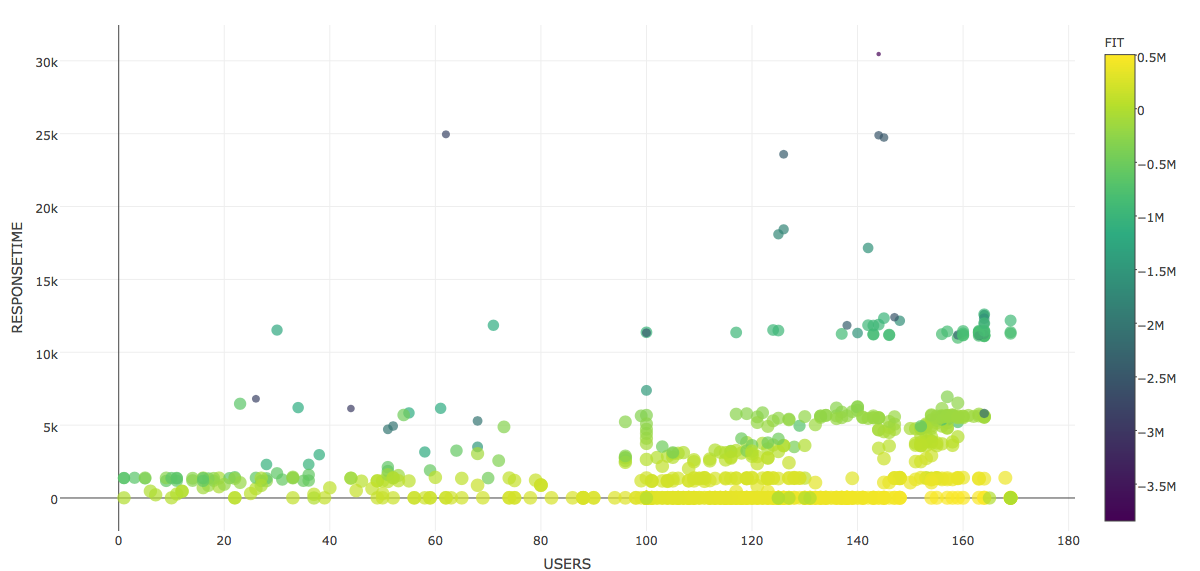
\includegraphics[width=1\textwidth]{./images/experiment1-7.png}
\caption{Response time by number of users of individuals with Happy Scenario 1 and Happy Scenario 2}
\label{fig:responsetimegenerationalltests1}
\end{figure}


Fig. \ref{fig:mdpexperiment1} presents the markov decision process for the experiment. When the response time it is bellow or equal the service level, the action with major reward it is increase the number of users and include more positions with the Happy Scenario 2 (Happy 2). When the response time is above the service level, the action with major reward value it is decrease the number of users and include more positions with the Happy Scenario 2. The actions  with minor value of reward contais the both antipatterns Circuitous Treasure (CTH) and The Ramp antipatterns (Ramp).

In the first experiment, We conclude that the metaheuristics converged to scenarios with an happy path, excluding the scenarios with antipatterns. The hybridQ and hybrid metaheuristic returned individuals with higher fitness scores. However, the Hybrid metaheuristic made twice as many requests than Tabu Search to overcome it. 

\begin{figure}[h]
\centering
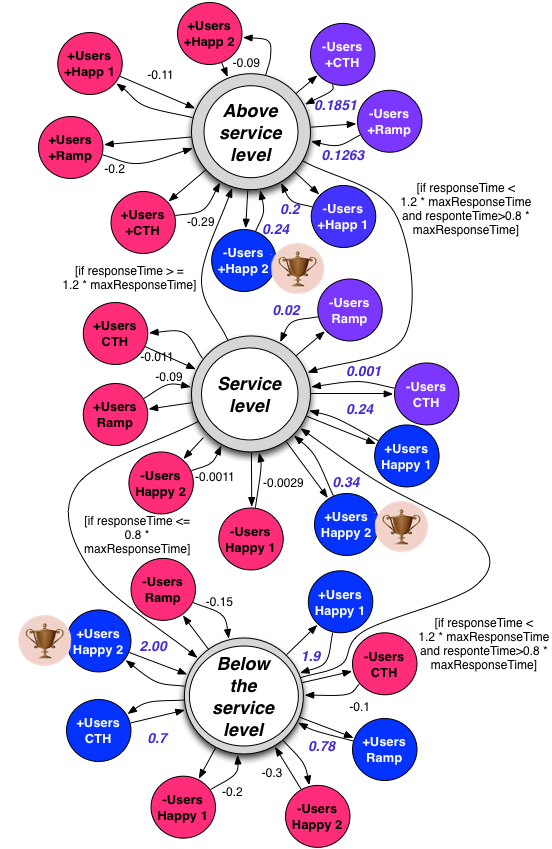
\includegraphics[width=0.6\textwidth]{./images/mdpexperiment.png}
\caption{Markov decision process of experiment with Circuitous Treasure and The Ramp antipatterns}
\label{fig:mdpexperiment1}

\end{figure}

\FloatBarrier
\subsection{The Tower Babel  and Unbalanced Processing experiment}

The experiment was carried out for 6 continuous hours. All tests in the experiment were conducted without the need of a tester. In this experiment, Scenarios were generated with Tower Babel and Unbalanced Processing antipattern as well as scenarios with Happy Scenario 1, Happy Scenario 2 and mixed scenarios. The Fig. \ref{fig:fitnessbygeneration2}  presents the fitness value obtained by each metaheuristic. The SA algorithm obtained the worst fitness values. Hybrid metaheuristic obtained the better fitness values.


\begin{figure}[h]
\centering
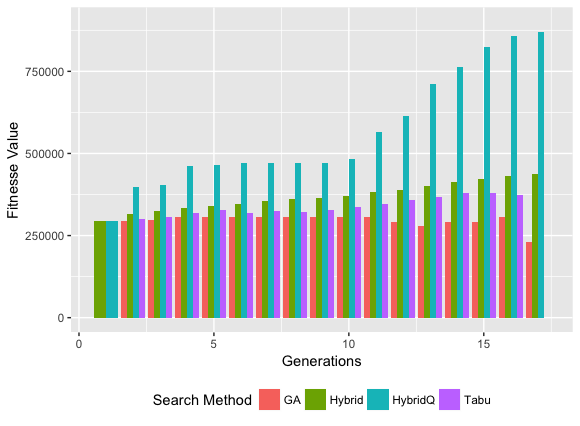
\includegraphics[width=.9\textwidth]{./images/experiment2-7.png}
\caption{Fitness value obtained by Search Method}
\label{fig:fitnessbygeneration2}
\end{figure}

As in the first experiment, the Hybrid algorithm performs twice as many requests as the second one, the tabu search (Fig. \ref{fig:numberofrequestsbysearchmethod2}). The Fig. \ref{fig:boxplot2} shows the average, minimal e maximum value by search method. The Fig. \ref{fig:summaryboxplot2} presents the maximum, average, median and minimum fitness value by generation. The maximun fitness value increases at each generation. The Fig. \ref{fig:density2} presents the density graph of number of users by fitness value. The range between 100 and 150 users has the highest number of individuals found with higher fitness value.


\begin{figure}[h]
\begin{minipage}{.5\textwidth}
\centering
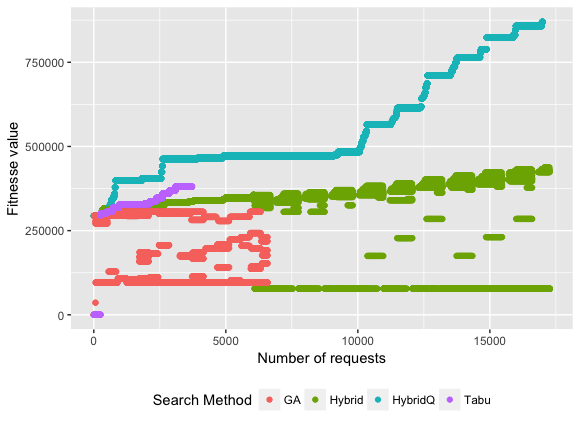
\includegraphics[width=1\textwidth]{./images/experiment2-1.png}
\caption{Number of requests by Search Method}
\label{fig:numberofrequestsbysearchmethod2}
\end{minipage}
\begin{minipage}{.5\textwidth}
\centering
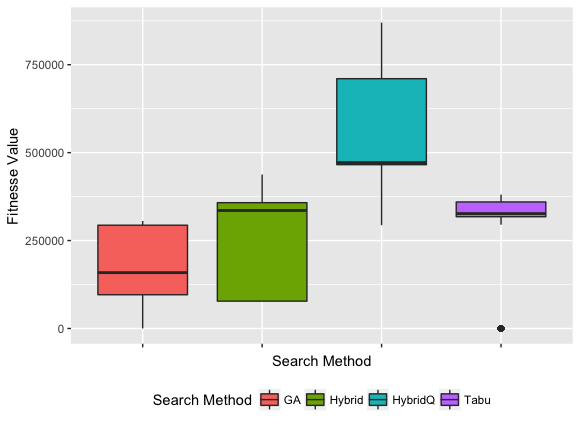
\includegraphics[width=1\textwidth]{./images/experiment2-2.png}
\caption{Fitness value by generation in all tests}
\label{fig:boxplot2}
\end{minipage}

\end{figure}



\begin{figure}[h]
\begin{minipage}{.5\textwidth}
\centering
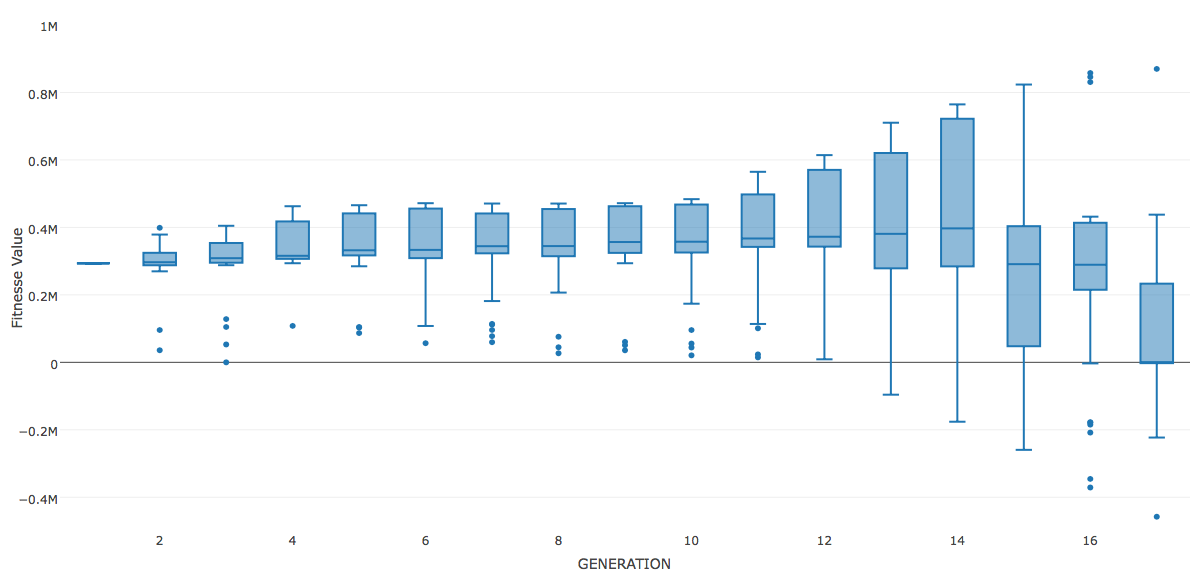
\includegraphics[width=1\textwidth]{./images/experiment2-3.png}
    \caption{Response time by generation in all tests scenarios}
\label{fig:summaryboxplot2}
\end{minipage}
\begin{minipage}{.5\textwidth}
\centering
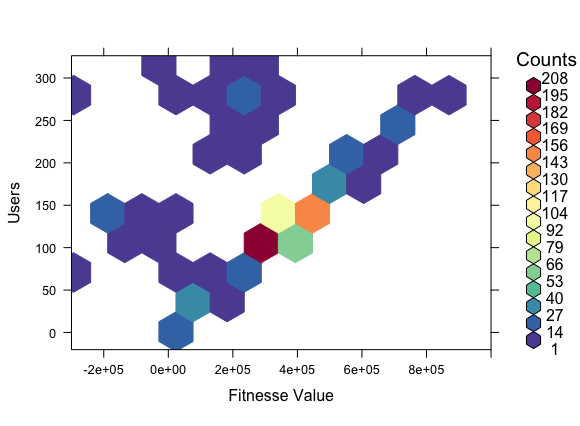
\includegraphics[width=1\textwidth]{./images/experiment2-4.png}
\caption{Finesse value by generation in all tests}
\label{fig:density2}
\end{minipage}

\end{figure}

Table \ref{tab:bestindividuals2} shows 4 individuals with 279 to 292 users.  The first individual has 121 users on Happy Scenario 2, 171 users on Happy Scenario 1 and a response time of 11 seconds. None of the best individuals found implements the Unbalanced Processing or Tower Babel antipattern.

Fig. \ref{fig:responsetimegenerationalltests2} presents the response time by number of users of individuals with Happy Scenario 1 and Happy Scenario 2. The Figure illustrates that the individuals with best fitness value has more users and minor response time. The Fig. \ref{fig:fitnessgenerationalltests2-1} presents the response time by number of users of individuals with with Unbalanced Processing and Tower Babel antipatterns scenarios. The Figure illustrates the smallest number of individuals with the  Unbalanced Processing and Tower Babel antipattern when compared to individuals who use the happy scenarios and the Tower Babel antipattern.



\begin{figure}[h]
\centering
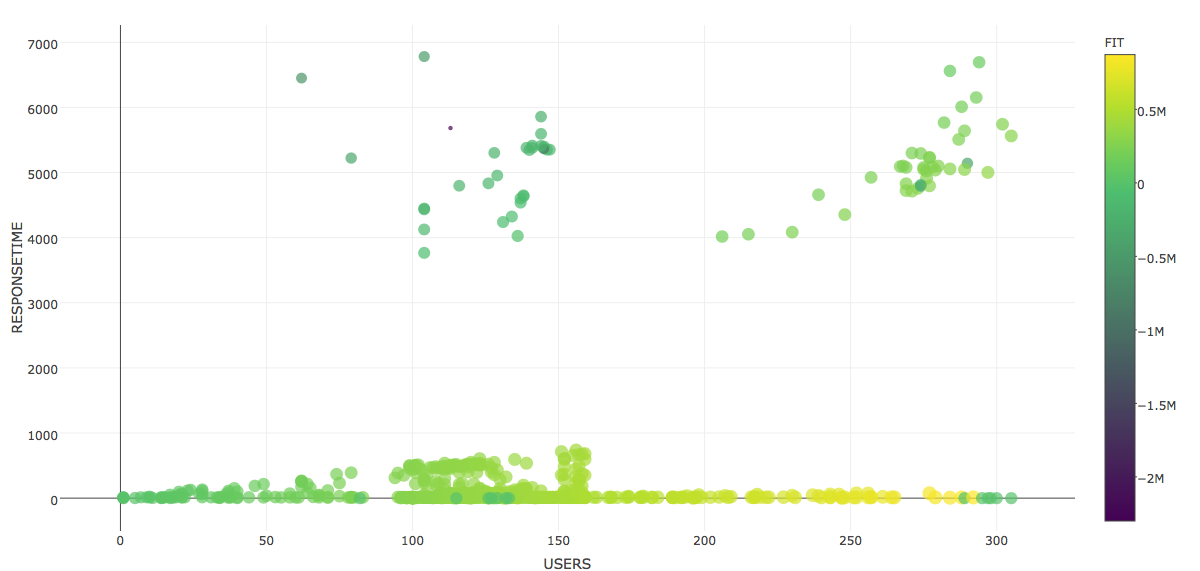
\includegraphics[width=1\textwidth]{./images/experiment2-5.png}
\caption{Response time by number of users of individuals with Happy Scenario 1, Happy Scenario 2 and Tower Babel antipattern}
\label{fig:responsetimegenerationalltests2}
\end{figure}


\begin{figure}[h]
\centering
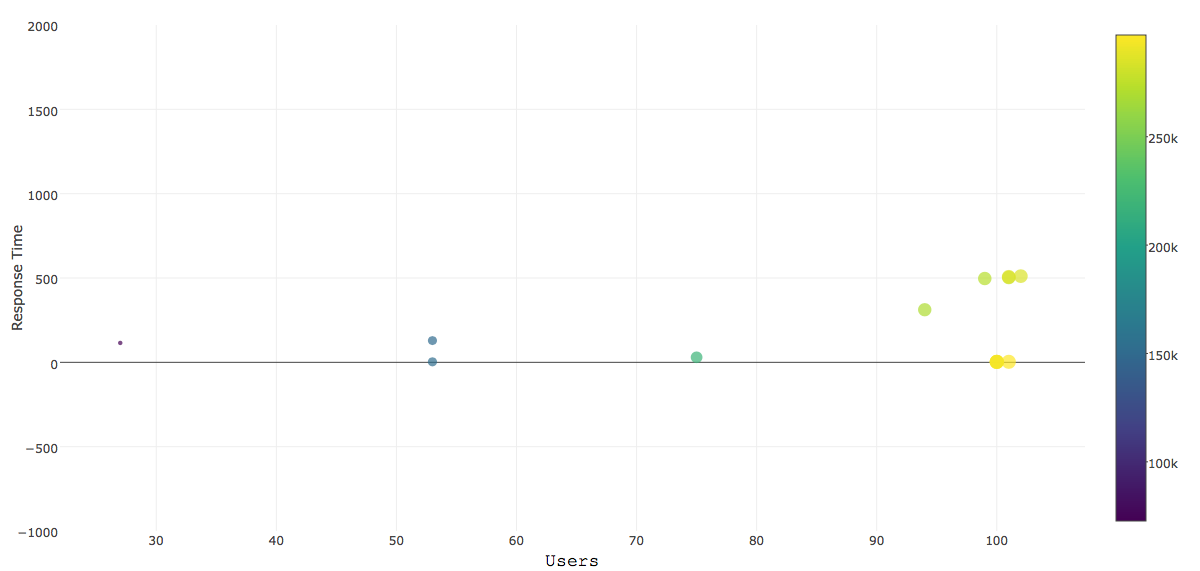
\includegraphics[width=1\textwidth]{./images/experiment2-6.png}
\caption{Response time by number of users of individuals with Unbalanced Processing antipattern}
\label{fig:fitnessgenerationalltests2-1}
\end{figure}


We conclude that the metaheuristics converged to scenarios with an happy path, excluding the scenarios with Unbalanced Processing and Tower Babel antipattern. The hybrid metaheuristic with Q-Learning (HybridQ) returned individuals with higher fitness scores. The Hybrid metaheuristic (Hybrid) made twice as many requests than Tabu Search to overcome it. The SA algorithm obtained the worst fitness values. The algorithm initially used a scenario with an antipattern and found neighbors that still using an antipattern over the 17 generations of the experiment. The individual with best fitness value has 121 users on Happy Scenario 2, 171 users on Happy Scenario 1 and a response time of 11 seconds.

% Please add the following required packages to your document preamble:
% \usepackage[table,xcdraw]{xcolor}
% If you use beamer only pass "xcolor=table" option, i.e. \documentclass[xcolor=table]{beamer}
\begin{table}[h]
\centering
\caption{Best individuals found in the second experiment}
\label{tab:bestindividuals2}
\begin{tabular}{lllllll}
\rowcolor[HTML]{FFCCC9} 
\textbf{Search Method} & \textbf{Generation} & \textbf{Users} & \textbf{fitness Value} & \textbf{Happy 2} & \textbf{Happy 1} & \textbf{Time} \\ 
\multicolumn{1}{l}{HybridQ} & \multicolumn{1}{l}{17} & \multicolumn{1}{l}{292} & \multicolumn{1}{l}{869780}  & \multicolumn{1}{l}{121} & \multicolumn{1}{l}{171} & \multicolumn{1}{l}{11} \\ 
\multicolumn{1}{l}{HybridQ} & \multicolumn{1}{l}{16} & \multicolumn{1}{l}{288} & \multicolumn{1}{l}{857780} &  \multicolumn{1}{l}{103} & \multicolumn{1}{l}{185} & \multicolumn{1}{l}{11} \\ 
\multicolumn{1}{l}{HybridQ} & \multicolumn{1}{l}{16} & \multicolumn{1}{l}{284} & \multicolumn{1}{l}{845880} &  \multicolumn{1}{l}{167} & \multicolumn{1}{l}{117} & \multicolumn{1}{l}{10} \\ 
\multicolumn{1}{l}{HybridQ} & \multicolumn{1}{l}{16} & \multicolumn{1}{l}{279} & \multicolumn{1}{l}{830780} &  \multicolumn{1}{l}{144} & \multicolumn{1}{l}{135} & \multicolumn{1}{l}{11} \\ 
\end{tabular}
\end{table}


\section{JPetStore Application Experiments}

Two experiments were conducted to test the use of the HybridQ algorithm in a real implemented application. The chosen application was the JPetStore, available at \url{https://hub.docker.com/r/pocking/jpetstore/}. The maximum tolerated response time in the test was 10 seconds.  Any  individuals who obtained a time longer than the stipulated maximum time suffered penalties.  The whole process of stress and performance tests, which took 2 days and about 1800 executions, was carried out without the need for monitoring by a test designer. The tool automatically selected the next scenarios to be run up to the limit of eleven generations previously established. The experiments use the follow application features:


\begin{itemize}
\item Enter in the Catalog: the application presents the catalog of pets.
\item Fishs: The application shows the recorded fishs items.
\item Register:  a new user realize the register in the system.
\item Dogs: The application shows the recorded dogs items.
\item Shopping Cart: the application presents the shopping cart.
\item Add or Remove in Shopping Cart: the application adds and removes items from shopping cart.
\end{itemize}


The experiment used the following fitness function:

\begin{equation}
\begin{aligned}
fitness=\begin{cases} n*\{3000*numberOfUsers-20* 90percentiletime-20*80percentiletime\\-20*70percentiletime
-20*maxResponseTime-penalty\} , \textsf{where n is the }\\\ \textsf{ number of features used by the test in a set of previous selected application} \\ \textsf{features}
\end{cases}
\end{aligned}
\end{equation}


The purpose of the fitness function is to maximize the number of users and minimize the response time in the tests containing the selected functionalities. For example, it is possible double the fitness value for tests that have the fish lookup feature and user registration.

\subsection{JPetStore  Cart and Register experiment }

This first experiment tries to find the scenarios with maximal number of users and best response time tests that contains the Cart and Register features. The Fig. \ref{fig:experiment31} and \ref{fig:experiment32} show the fitness value by generation. The HybridQ obtained the best fitness values in all generations.

\begin{figure}[h]
\begin{minipage}{.5\textwidth}
\centering
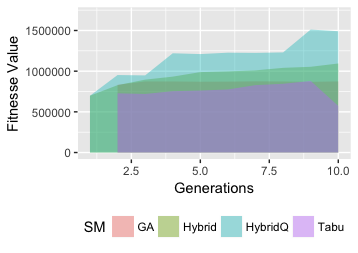
\includegraphics[width=1\textwidth]{./images/experiment3-1.png}
\caption{Fitness value by generation on JPetStore First experiment}
\label{fig:experiment31}
\end{minipage}
\begin{minipage}{.5\textwidth}
\centering
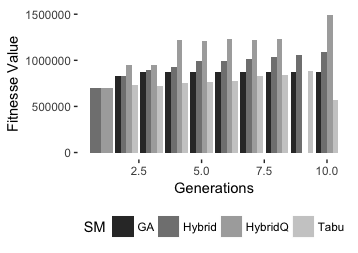
\includegraphics[width=1\textwidth]{./images/experiment3-2.png}
\caption{Fitness value by generation on JPetStore First experiment}
\label{fig:experiment32}
\end{minipage}
\end{figure}

The Fig. \ref{fig:numberofrequestsbysearchmethod3} shows the fitness value by number of request by each Search Method. In the Figure, it is possible to observe that HybridQ obtained the best fitness value to same number of requests of the other algorithms.

\begin{figure}[h]
\begin{minipage}{.5\textwidth}
\centering
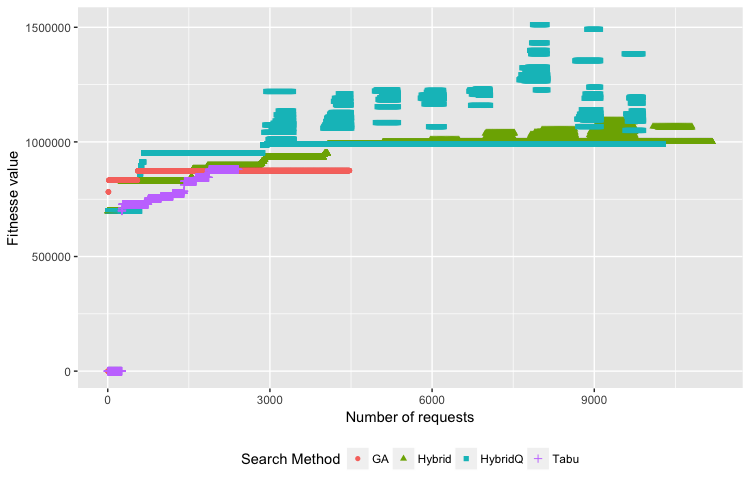
\includegraphics[width=1\textwidth]{./images/experiment3-3.png}
\caption{Number of requests by Search Method}
\label{fig:numberofrequestsbysearchmethod3}
\end{minipage}
\begin{minipage}{.5\textwidth}
\centering
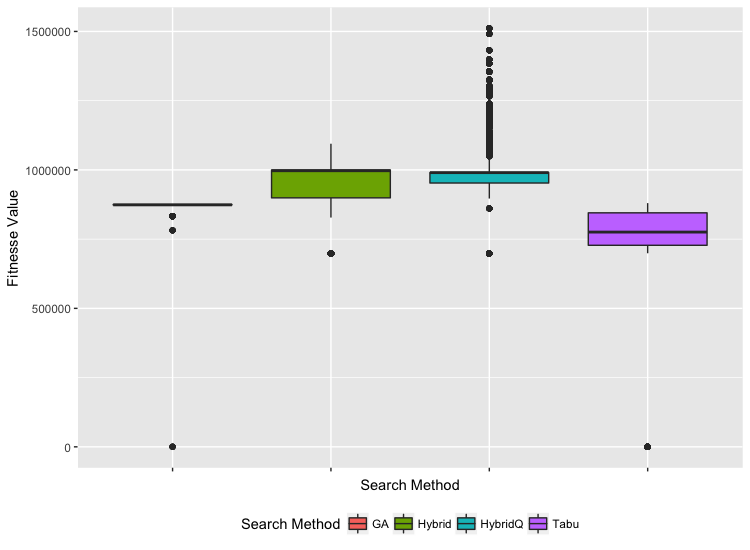
\includegraphics[width=1\textwidth]{./images/experiment3-4.png}
\caption{Fitness value by generation in all tests}
\label{fig:boxplot3}
\end{minipage}

\end{figure}

The Fig. \ref{fig:summaryboxplot3} presents the maximum, average, median and minimum fitness value by generation. The maximun fitness value increases at each generation. Table \ref{tab:bestindividuals3} shows 4 individuals with 233 to 398 users.  The first individual has 73 users on Fishs scenario, 17 users on Dogs scenario, 50 users on Cart scenario, 33 Users on register scenario  and a response time of 357 seconds. 

\begin{figure}[h]
\centering
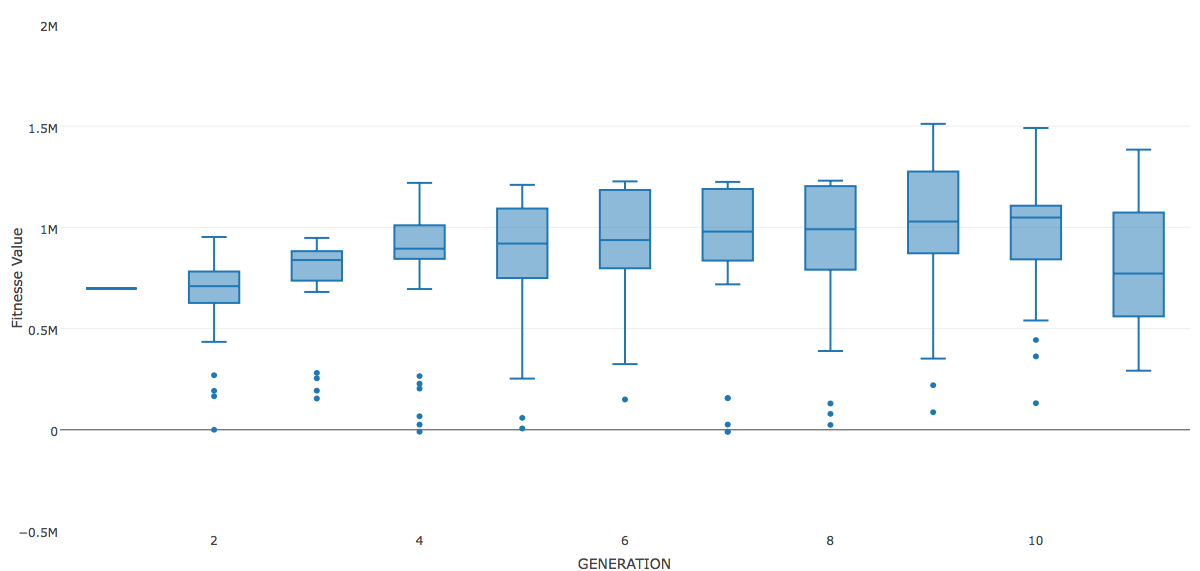
\includegraphics[width=1\textwidth]{./images/experiment3-5.png}
\caption{Average, median and minimum fitness value by Search Method }
\label{fig:summaryboxplot3}
\end{figure}




% Please add the following required packages to your document preamble:
% \usepackage[table,xcdraw]{xcolor}
% If you use beamer only pass "xcolor=table" option, i.e. \documentclass[xcolor=table]{beamer}
\begin{table}[h!]
\centering
\caption{Best individuals found in JPetStore first experiment}
\label{tab:bestindividuals3}
\begin{tabular}{lllllllll}
\rowcolor[HTML]{C0C0C0} 
\textbf{Search Method} & \textbf{Response} & \textbf{Users} & \textbf{Gen} & \textbf{Fitness} & \textbf{Fishs} & \textbf{Dogs} & \textbf{Cart} & \textbf{Register} \\
HybridQ                & 357               & 173            & 9            & 44773            & 73             & 17            & 50            & 33                \\
HybridQ                & 398               & 171            & 10           & 44831            & 57             & 33            & 48            & 33                \\
HybridQ                & 331               & 164            & 9            & 44774            & 71             & 14            & 51            & 28                \\
HybridQ                & 233               & 159            & 9            & 44783            & 63             & 31            & 32            & 33               
\end{tabular}
\end{table}

We conclude that the individuals with major number of uses the four scenarios. The scenario with major number of users is the Fish search feature. The hybrid metaheuristic with Q-Learning (HybridQ) returned individuals with higher fitness scores.  The individual with best fitness value has 73 users on Fishs scenario, 17 users on Dogs scenario, 50 users on Cart scenario, 33 Users on register scenario  and a response time of 357 seconds. 






%\begin{acknowledgements}
%If you'd like to thank anyone, place your comments here
%and remove the percent signs.
%\end{acknowledgements}

% BibTeX users please use one of
%\bibliographystyle{spbasic}      % basic style, author-year citations
%\bibliographystyle{spmpsci}      % mathematics and physical sciences
%\bibliographystyle{spphys}       % APS-like style for physics
%\bibliography{}   % name your BibTeX data base

% Non-BibTeX users please use
\begin{thebibliography}{}
%
% and use \bibitem to create references. Consult the Instructions
% for authors for reference list style.
%
\bibitem{RefJ}
% Format for Journal Reference
Author, Article title, Journal, Volume, page numbers (year)
% Format for books
\bibitem{RefB}
Author, Book title, page numbers. Publisher, place (year)
% etc
\end{thebibliography}

\end{document}
% end of file template.tex

